\graphicspath{{Figures/}}

\title{\fontsize{33}{45}{\huge Pattern Classification (EET 3035)\newline \vspace{8pt} \Large Lecture 01\vspace{-1.1cm}}}
\author{\vspace{-0.4cm}\\\normalsize{\bf Dr. Kundan Kumar}\\ PhD (IIT Kharagpur)\\
Associate Professor\\Department of ECE}
% - Give the names in the same order as the appear in the paper.
% - Use the \inst{?} command only if the authors have different
%   affiliation.

\institute[Indian Institute of Technology Kharagpur] % (optional, but mostly needed)
{

\includegraphics[height=.17\textheight]{SOAlogo.png}\\
 Faculty of Engineering (ITER)\\ S`O'A Deemed to be University, Bhubaneswar, India-751030\\
 \copyright\  2020 Kundan Kumar, All Rights Reserved\\
  \vspace{-1.1cm}}
% - Use the \inst command only if there are several affiliations.
% - Keep it simple, no one is interested in your street address.
\date{}
% To remove page number from a perticular slide
{
\setbeamertemplate{logo}{}
\makeatletter
\setbeamertemplate{footline}{
        \leavevmode%
  
  % First line.
  \hbox{%
  \begin{beamercolorbox}[wd=.2\paperwidth,ht=\beamer@decolines@lineup,dp=0pt]{}%
  \end{beamercolorbox}%
  \begin{beamercolorbox}[wd=.8\paperwidth,ht=\beamer@decolines@lineup,dp=0pt]{lineup}%
  \end{beamercolorbox}%
  } %
  % Second line.
  \hbox{%
  \begin{beamercolorbox}[wd=\paperwidth,ht=\beamer@decolines@linemid,dp=0pt]{linemid}%
  \end{beamercolorbox}%
  } %
  % Third line.
  \hbox{%
  \begin{beamercolorbox}[wd=.1\paperwidth,ht=\beamer@decolines@linebottom,dp=0pt]{}%
  \end{beamercolorbox}%
  \begin{beamercolorbox}[wd=.9\paperwidth,ht=\beamer@decolines@linebottom,dp=0pt]{linebottom}%
  \end{beamercolorbox}%
  }%
        }
\makeatother
\begin{frame}
\titlepage
\end{frame}
}

\section{Text books and Syllabus}
\subsection{}

\begin{frame}[label=12]{Outline}
\tableofcontents
\end{frame}

\begin{frame}{Text Books and Credits}
%\vspace{-0.5cm}
\begin{columns}
\begin{column}{5cm}
\begin{figure}
\centering
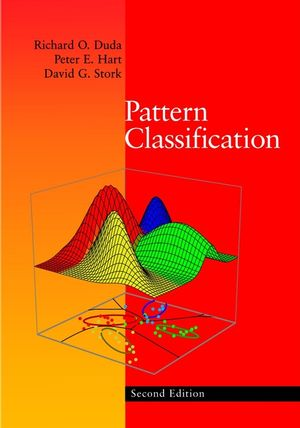
\includegraphics[height = 3cm,width = 2.2cm]{PatternBook.jpg}~~
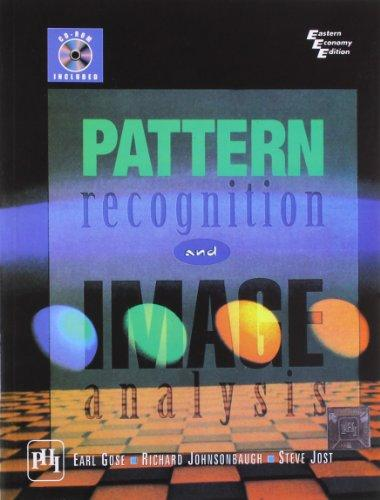
\includegraphics[height = 3cm,width = 2.2cm]{GoseBook.jpg}\\
\vspace{8pt}
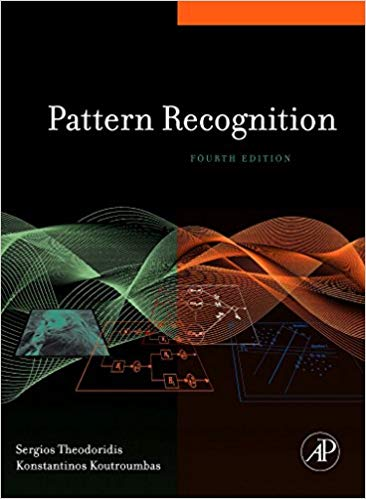
\includegraphics[height = 3cm,width = 2.2cm]{Figures/Book003.jpg}~~
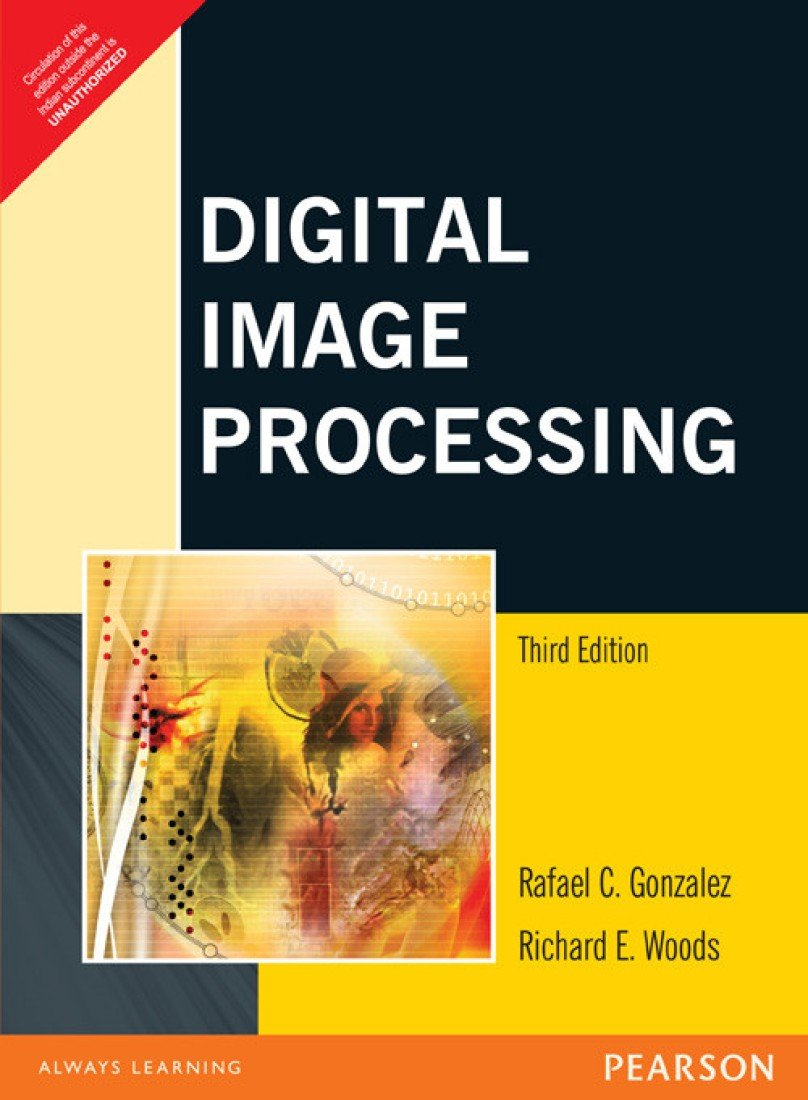
\includegraphics[height = 3cm,width = 2.2cm]{Figures/Book004.jpg}
\end{figure}
\end{column}
\begin{column}{5.4cm}
\begin{footnotesize}
\textbf{Text Book:}
\begin{itemize}
\item Pattern Classification, Duda-Hart, 2nd Edition ({\color{brown}Prescribed})
\item Pattern Recognition and Image Analysis by Earl Gose
\item Pattern Recognition by Theodoridis, 4th Edition
\item Digital Image Processing by Gonzalez, 3rd Edition
\end{itemize}
\textbf{Credits:}
\begin{itemize}
\item 4 credits course, 4 Classes/week (1hr/Class)
\item Prerequisite: MTH 2002 (Probability and Statistics)
\end{itemize}
\end{footnotesize}
\end{column}
\end{columns}
\end{frame}

\begin{frame}{Grading Pattern and Syllabus}
\begin{itemize}
\item \textbf{Grading pattern}: 6
\begin{table}[h]
\begin{small}
\centering
\begin{tabular}{|L{4cm}C{0.6cm}L{2cm}|}
\hline
Attendance & : & 5 Marks  \\ \hline
2 Quizzes  & : & 10 Marks   \\  \hline
Assignments  & : & 10 Marks   \\  \hline
Mid-term examination & : & 15 Marks   \\ \hline
\textbf{Total Internal} & : & \textbf{40 Marks}   \\ \hline 
\multicolumn{3}{c}{}\\\hline
Theory examination  & : & 60 Marks   \\     \hline
\textbf{Total External} & : & \textbf{60 Marks} \\  \hline
\end{tabular}
\end{small}
\end{table}
\item \textbf{Syllabus:} Introduction, Features, Bayesian Decision Theory, Maximum Likelihood and Bayesian Parameter Estimation, Non-parameteric Techniques, Linear Discriminant Functions, Multilayer Neural Networks, Unsupervised learning and Clustering
\end{itemize}
\end{frame}

%\begin{frame}{In this course we are going to cover}
%%\setlength{\columnsep}{-2.1in}
%%  \begin{multicols}{2}
%    \begin{itemize}
%      \item Introduction to pattern recognition
%      \item Feature Extraction
%      \item Bayesian Decision Theory
%      
%      \item Normal Density
%      \item Discriminant Functions for the Normal Density
%      
%      \item Maximum Likelihood Parameter Estimation
%      \begin{itemize}
%      \item Component Analysis Discriminants
%      \end{itemize}
%      \item Non-parametric Techniques
%      \begin{itemize}
%      \item K-Nearest Neighbor Classification
%      \end{itemize}
%      \item Linear Discriminant Functions
%      \end{itemize}
%      \end{frame}
%      
%      \begin{frame}{In this course we are going to cover}
%     \begin{itemize}
%      \item Multilayer Neural Networks (NN)
%      \begin{itemize}
%      \item Perceptron Criterion
%      \item Feed-Forward Back-propagation NN
%      \item Radial Basis Function NN
%      \item Support Vector Machine
%      \end{itemize}
%      \item Unsupervised Learning and Clustering
%      \begin{itemize}
%      \item Agglomerative Clustering
%      \item Graph Based Clustering
%      \item Clustering Using Minimal Spanning Tree
%      \item Iterative Clustering (K-means)
%      \item Criterion Function based Clustering
%      \end{itemize}
%    \end{itemize}
%%  \end{multicols}
%\end{frame}

\begin{frame}{Google Classrooms}
\begin{normalsize}
\begin{itemize}
\item All the communication will be through {\color{mycolor2}Google Classroom}:
\begin{itemize}
\item Course materials
\item Assignments
\item Announcements and Notices
\end{itemize}
\item join the course at {\color{blue}\url{https://classroom.google.com/}}
\item  {\color{mycolor2}Class Code} for section C: 
\begin{figure}
\centering

\includegraphics[scale=0.2]{Figures/courseCode}
\end{figure}
\item  {\color{mycolor2}Class Code} for section D: 
\begin{figure}
\centering

\includegraphics[scale=0.2]{Figures/ClassCode_ECE-D}
\end{figure}
\item Would you like to {\color{mycolor1}code in Python} for the topics to be covered in Pattern Classification?
\end{itemize}
\end{normalsize}
\end{frame}


\section{Introduction}
\subsection{}
\begin{frame}{}
\begin{variableblock}{\centering \Large \textbf{\vspace{4pt}\newline Introduction to Pattern Classification\vspace{4pt}}}{bg=slidecolor,fg=white}{bg=slidecolor,fg=white}
\end{variableblock}
\begin{figure}
\centering
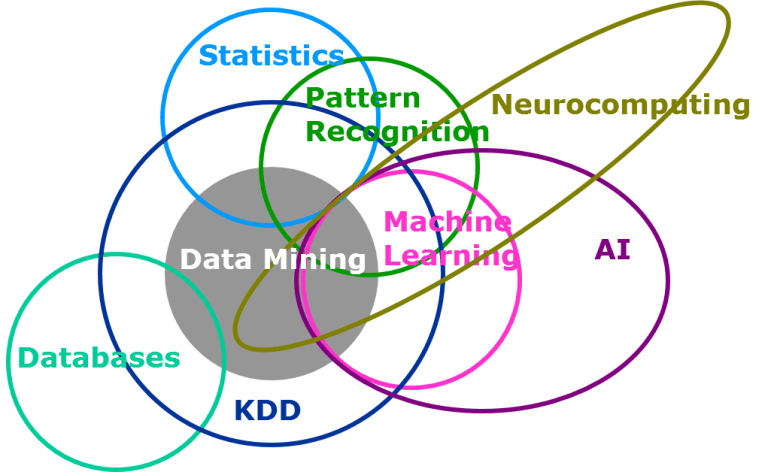
\includegraphics[width=0.7\textwidth]{Figures/domain.png}
\end{figure}
\end{frame}

\begin{frame}{Relation with AI and ML}
\begin{footnotesize}
\begin{itemize}
\item \textbf{\color{mycolor1}Artificial Intelligence}\\
\begin{itemize}
\item The {\color{mycolor2}theory and development of computer systems} able to perform tasks normally requiring {\color{mycolor4}human intelligence}, such as visual perception, speech recognition, decision-making, and translation between languages.  
\item {\color{mycolor2}Any technique which enables computers to mimic human behavior.} 
\end{itemize}
\item \textbf{\color{mycolor1}Machine learning} \\A field of computer science that uses statistical techniques to give computer systems {\color{mycolor4}the ability to "learn"} with data {\color{mycolor4}without being explicitly programmed} and {\color{mycolor2}progressively improve performance} on a specific task .
\item \textbf{\color{mycolor1}Pattern Classification}\\
\begin{itemize}
\item Pattern classification is a sub-topic of machine learning.
\item Pattern classification can be defined as a {\color{mycolor2}technique to classify data} (patterns) based either on a {\color{mycolor2}priori knowledge} or {\color{mycolor4}statistical information} extracted from the patterns.
\item Pattern recognition {\color{mycolor2}automatically discover the regularities} in data through the use of learning algorithms.
\end{itemize}
\end{itemize}
\end{footnotesize}
\end{frame}

\begin{frame}{Human Perception}
\begin{itemize}
\setlength{\itemsep}{20pt}
\item Humans have developed highly sophisticated skills for
sensing their environment and taking actions according to
what they observe, e.g.,
\begin{itemize}
\setlength{\itemsep}{5pt}
\item Recognizing a face,
\vspace{1.5cm}
\item Understanding spoken words,
\item Reading handwriting,
\vspace{1cm}
\item Distinguishing fresh food from its smell.
\end{itemize}
\item We would like to give similar capabilities to machines.
\end{itemize}

\begin{tikzpicture}[remember picture,overlay]
  \node (img1) at (2.5,5.1) {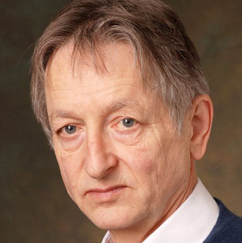
\includegraphics[height=1.3cm]{Figures/Hinton.jpg}};
   \node (img1) at (4,5.1) {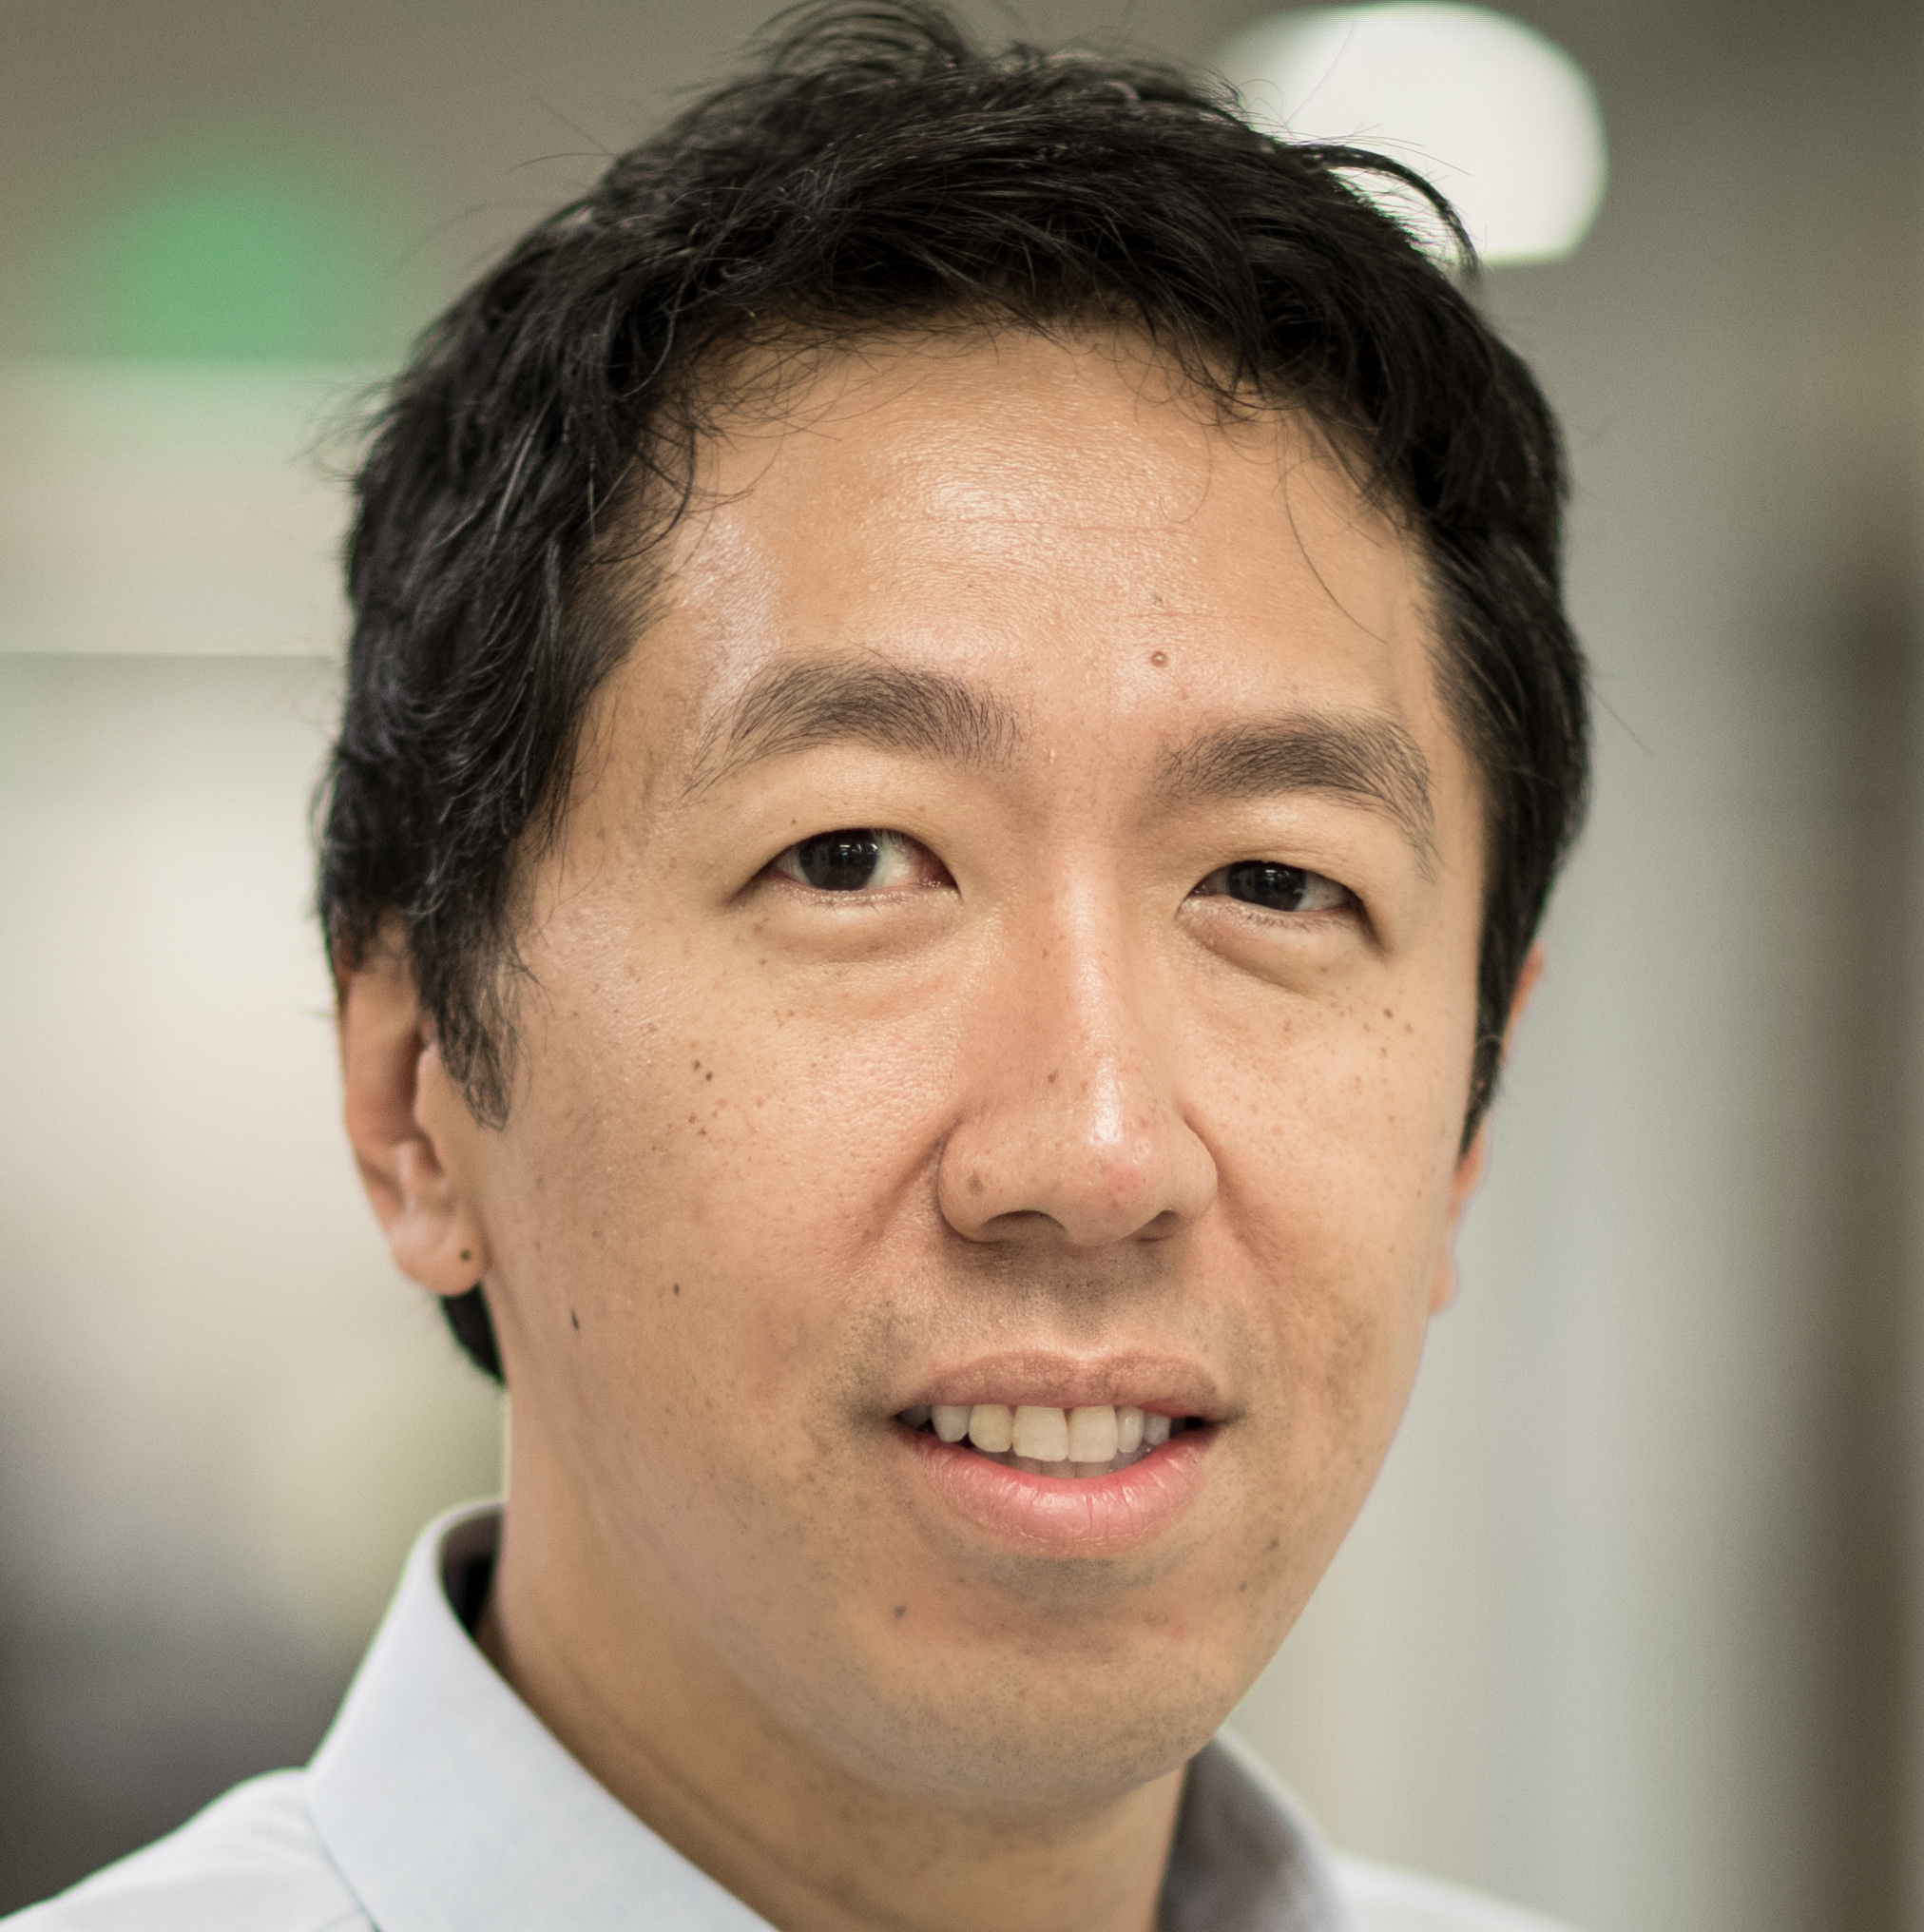
\includegraphics[height=1.3cm]{Figures/andrew.jpg}};
    \node (img1) at (5.5,5.1) {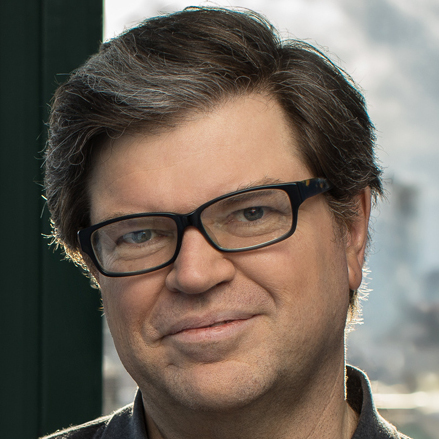
\includegraphics[height=1.3cm]{Figures/lecun.jpeg}};
      \node (img1) at (7,5.1) {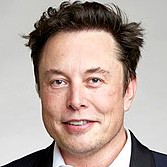
\includegraphics[height=1.3cm]{Figures/ElonMusk.jpg}};
   \onslide<2->{    \node (img1) at (8.5,5.1) {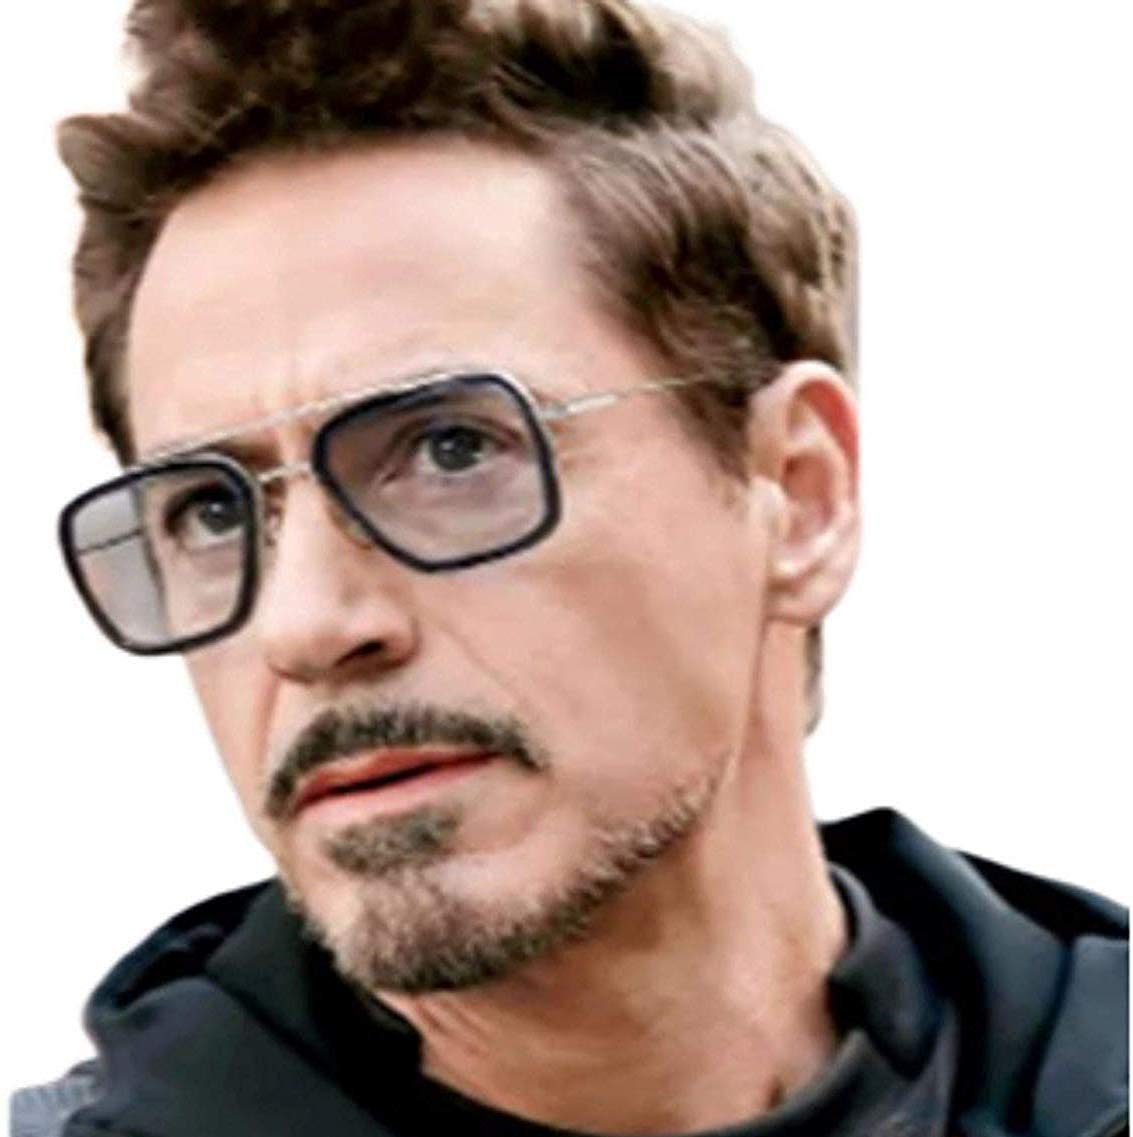
\includegraphics[height=1.3cm]{Figures/tonyStark.jpg}}; } 
  \onslide<3->{  \node (img1) at (4,2.7) {
\includegraphics[height=0.7cm]{Figures/digits.png}};}
\end{tikzpicture}
\end{frame}

\begin{frame}{What is Pattern Classification?}
\begin{figure}
\centering
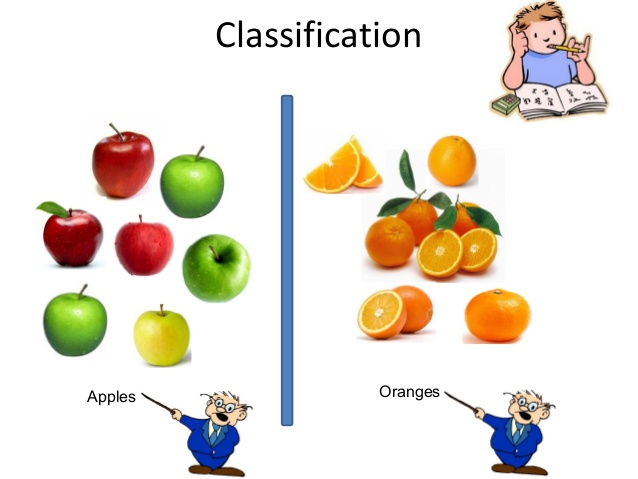
\includegraphics[scale=0.37]{AppleOrange.jpg}
\end{figure}
\end{frame}

\begin{frame}{What is Pattern Classification?}
\begin{itemize}
\item Assign an unknown pattern to one of several known categories (or classes).
\end{itemize}
\begin{figure}
\centering
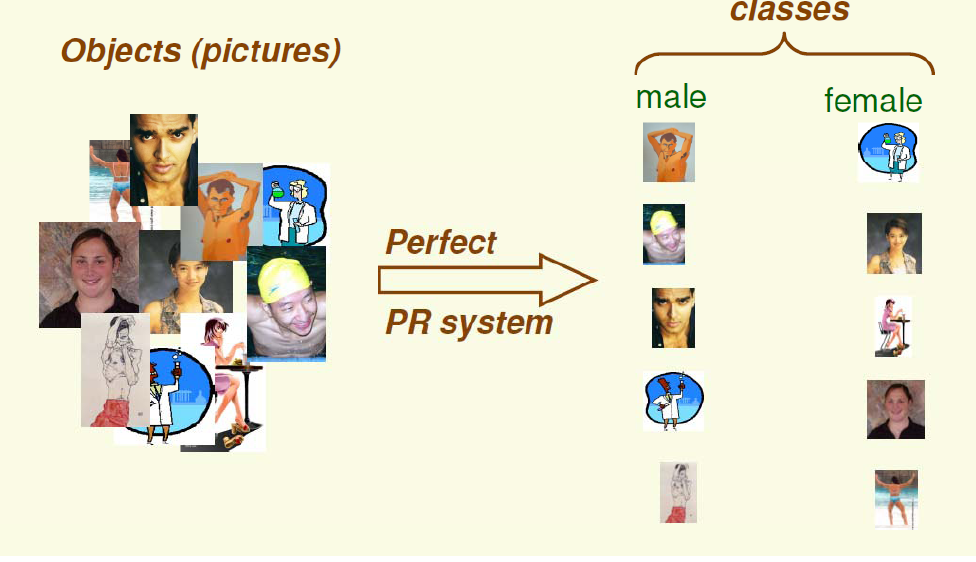
\includegraphics[scale=0.26]{Intro01.png}
\end{figure}
\end{frame}

\begin{frame}{What is a Pattern?}
\begin{itemize}
\item A pattern could be an \textbf{\color{mycolor2}object} or \textbf{\color{mycolor2}event}.
\end{itemize}
\begin{table}[]
\centering
\begin{tabular}{lc}
Biometric pattern & Hand gesture pattern  \\
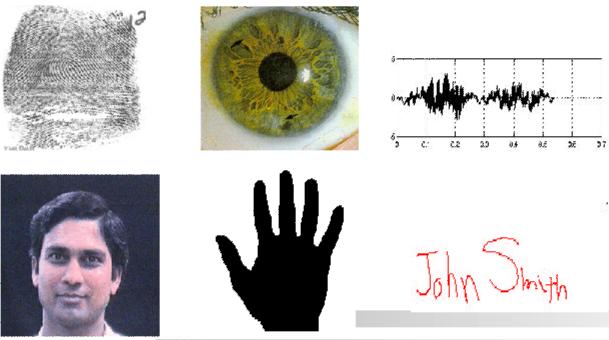
\includegraphics[scale=0.25]{Intro02} & 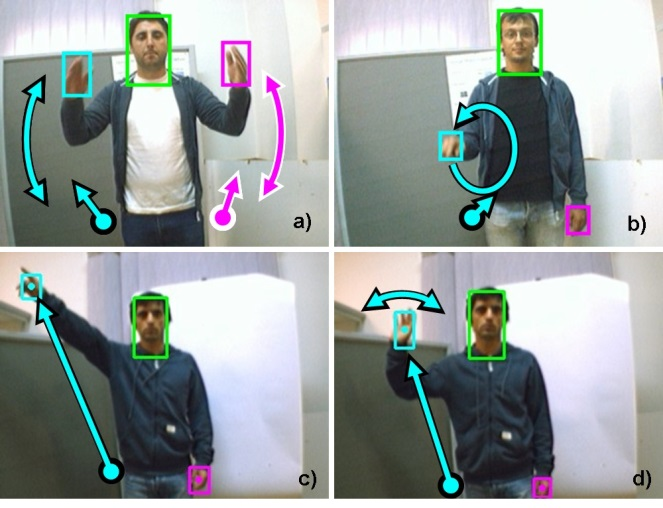
\includegraphics[scale=0.45]{Intro03} \\
\end{tabular}
\end{table}
\end{frame}

\begin{frame}{What is Pattern Classification?}
\begin{itemize}
\item A \textbf{\color{mycolor2}pattern} is an entity, vaguely defined, that could be given a name, e.g.,
\begin{itemize}
\item fingerprint image,
\item handwritten word,
\item human face,
\item speech signal,
\item DNA sequence,
\item $\ldots$
\end{itemize}
\item \textbf{\color{mycolor2}Pattern classification} is the study of how machines can
\begin{itemize}
\item observe the environment,
\item learn to distinguish patterns of interest,
\item make sound and reasonable decisions about the categories of the patterns.
\end{itemize} 
\end{itemize}
\end{frame}

\begin{frame}{Pattern Class}
\begin{itemize}
\item A collection of ``{\color{mycolor2} similar}'' objects.
\end{itemize}
\begin{table}[]
\centering
\begin{tabular}{c|clll}
Female & Male &  &  &  \\
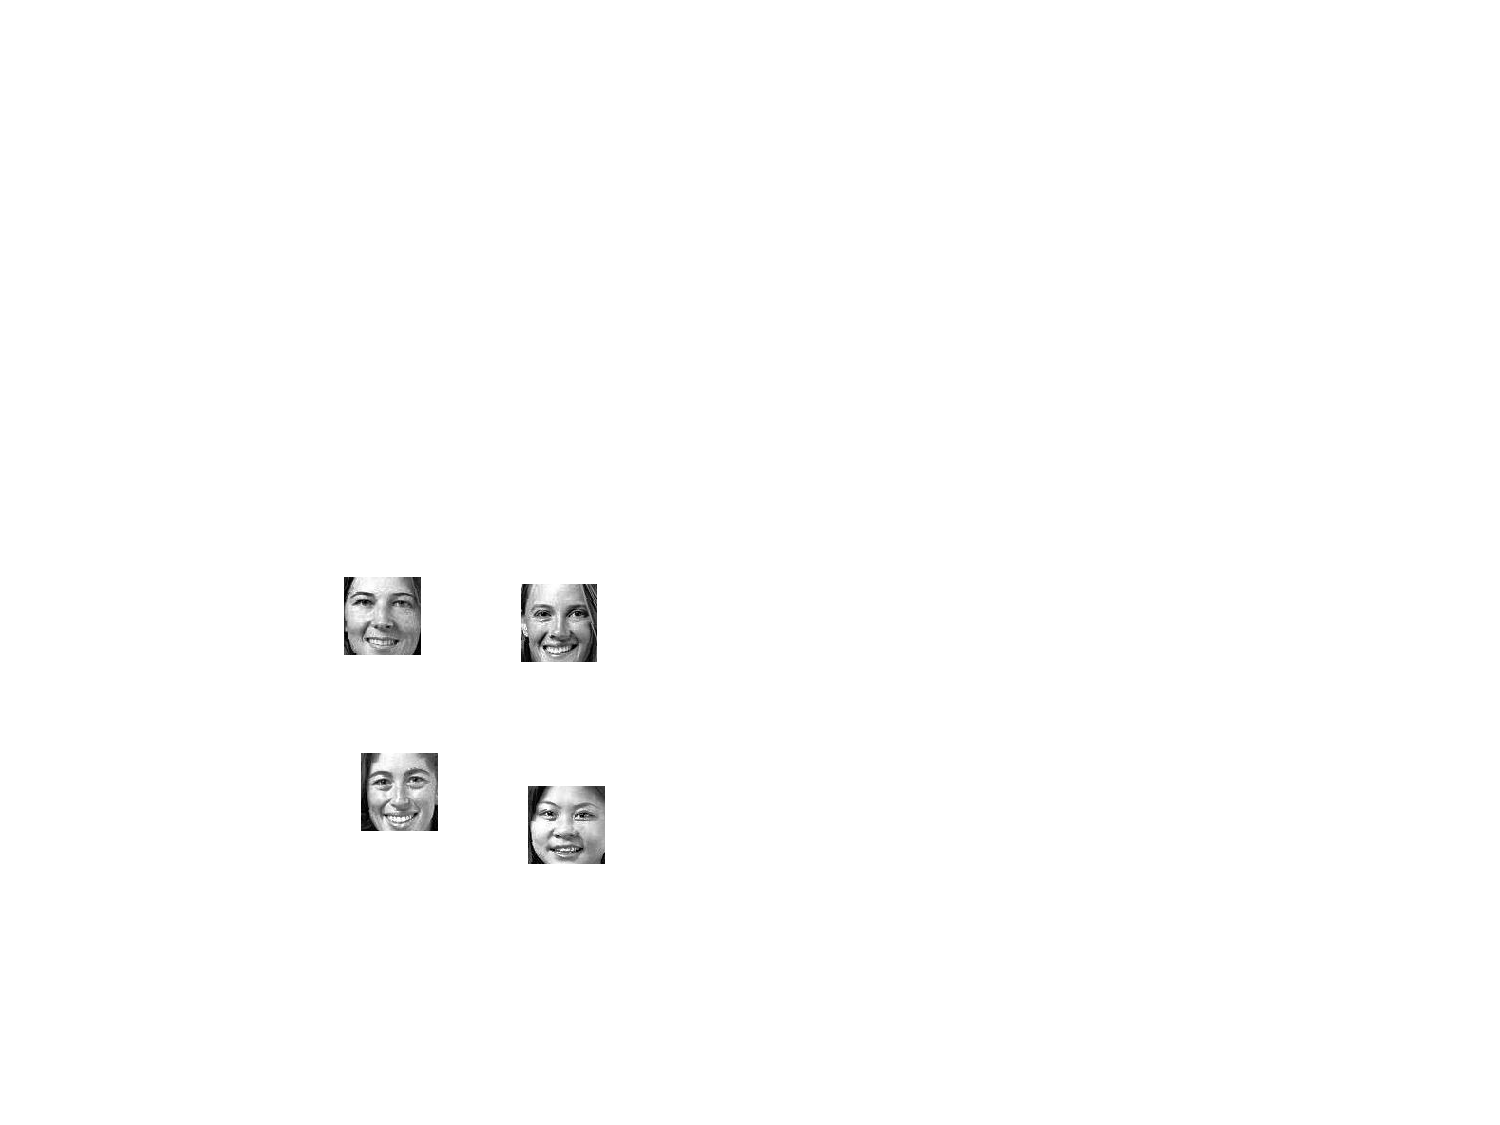
\includegraphics[scale=0.6]{Intro04} & 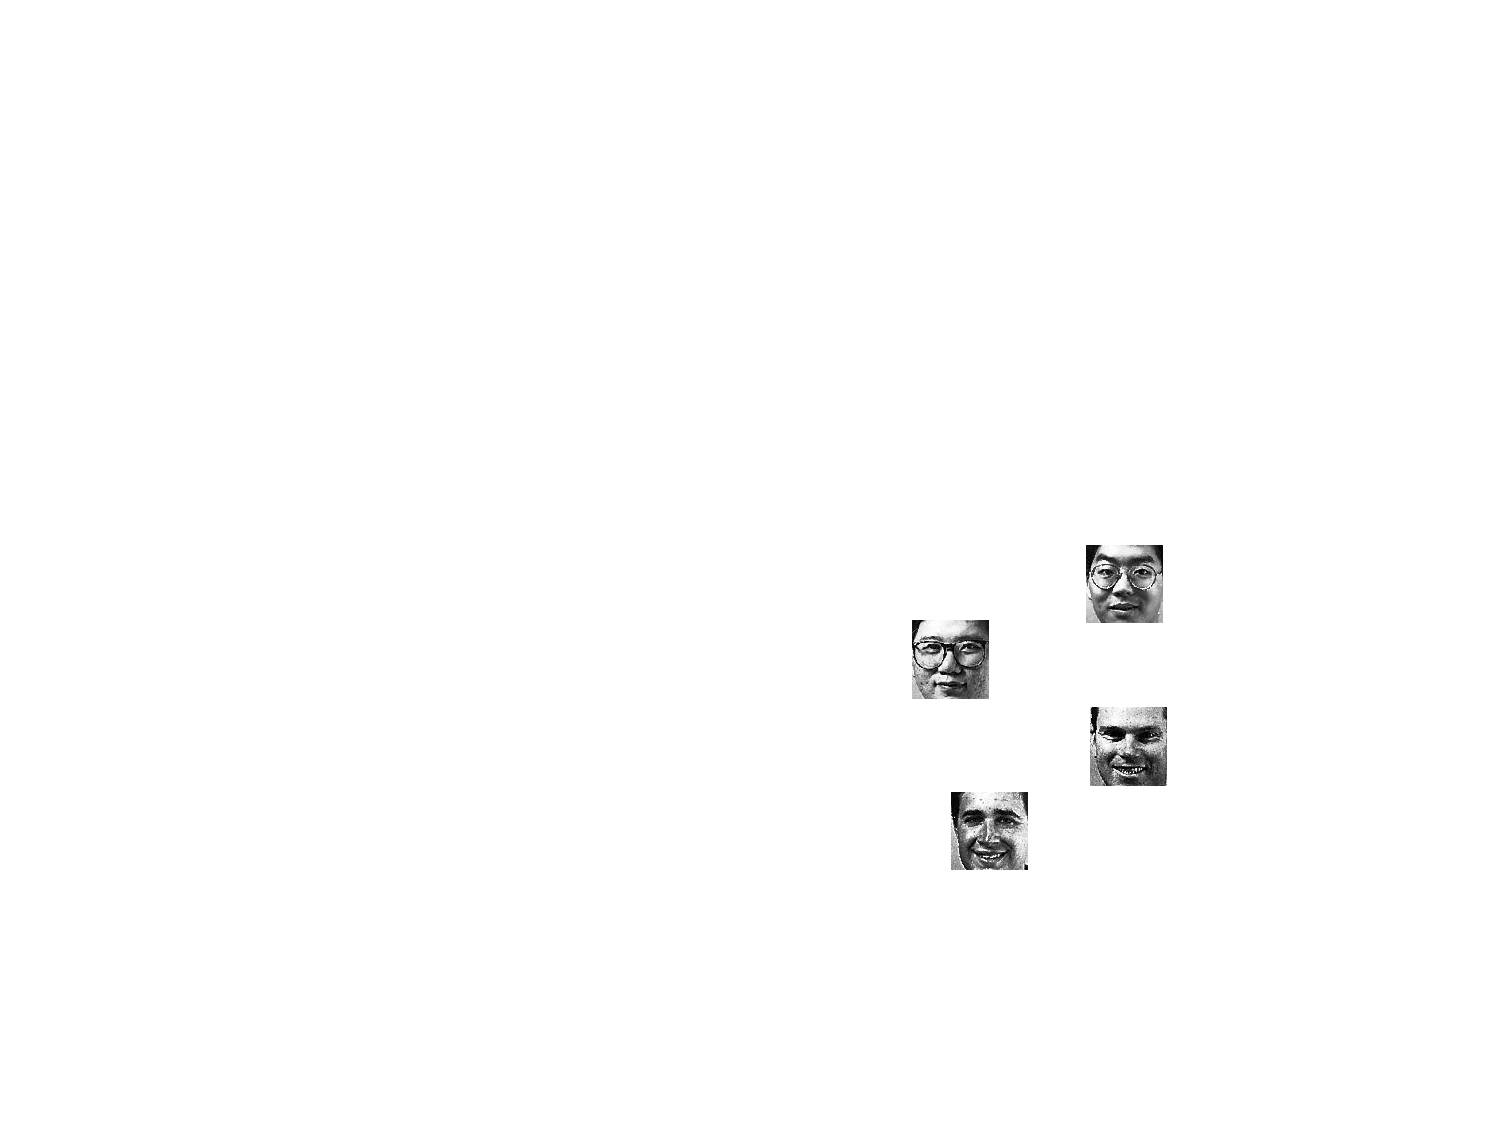
\includegraphics[scale=0.6]{Intro05} &  &  &  \\
  &   &  &  &  \\
  &   &  &  & 
\end{tabular}
\end{table}
\end{frame}

\begin{frame}{How do we model a Pattern Class?}
\begin{itemize}
\item Typically, using a statistical model.
\item Probability density function (e.g., Gaussian)
\end{itemize}
\begin{figure}
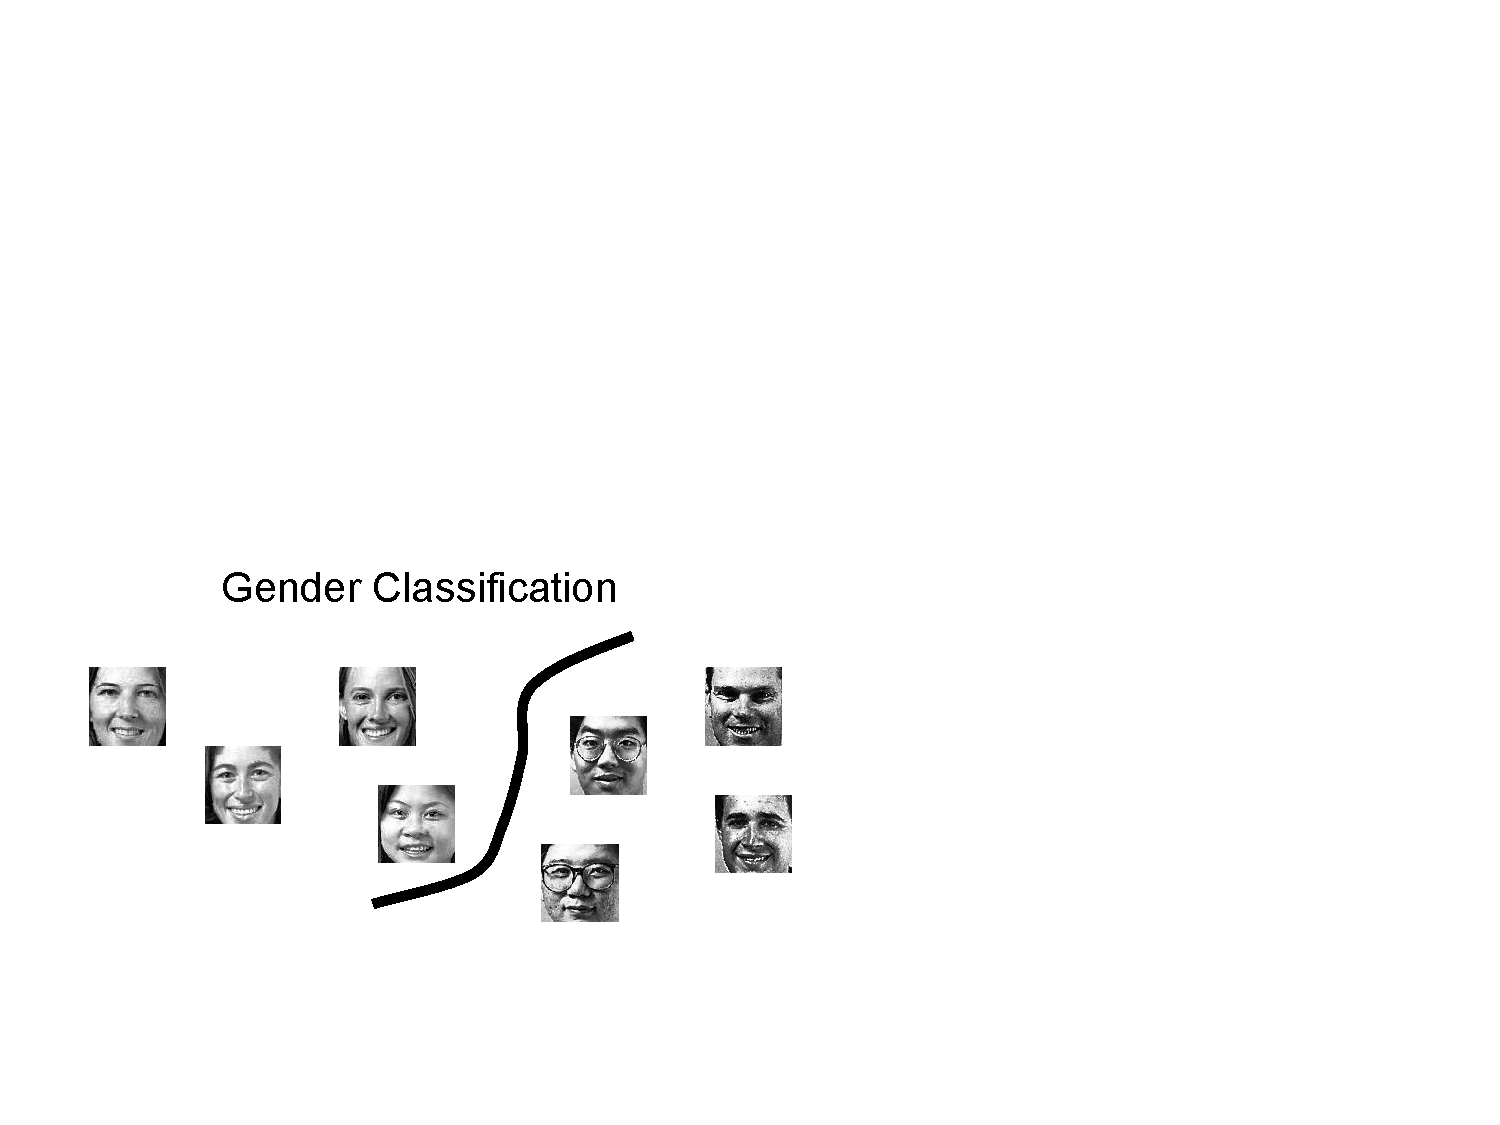
\includegraphics[width=6cm]{Figures/Intro06}~~~~
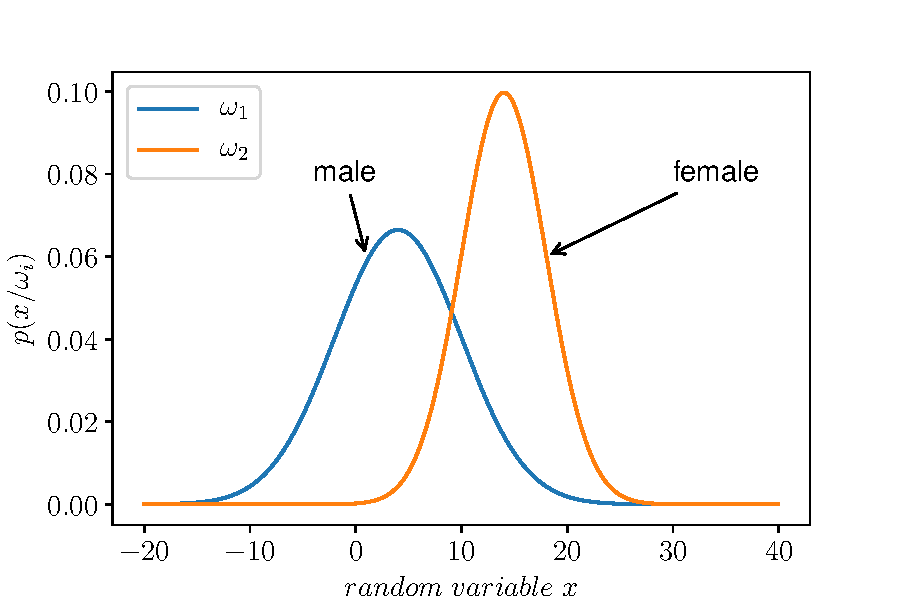
\includegraphics[width=5cm]{Figures/classProb}
\end{figure}
\end{frame}

\section{Applications}
\subsection{}

\begin{frame}{}
\begin{variableblock}{\centering \Large \textbf{\vspace{4pt}\newline Applications\vspace{4pt}}}{bg=slidecolor,fg=white}{bg=slidecolor,fg=white}
\end{variableblock}
\end{frame}

\begin{frame}{Machine Perception}
Build a machine that can recognize patterns:
\begin{itemize}
\item Speech recognition
\item Biometric recognition
\item Fingerprint identification
\item Face recognition
\item OCR (Optical Character Recognition)
\item DNA sequence identification
\item Autonomous navigation
\end{itemize}
\end{frame}

\begin{frame}{Applications: Speech Recognition}
\begin{figure}
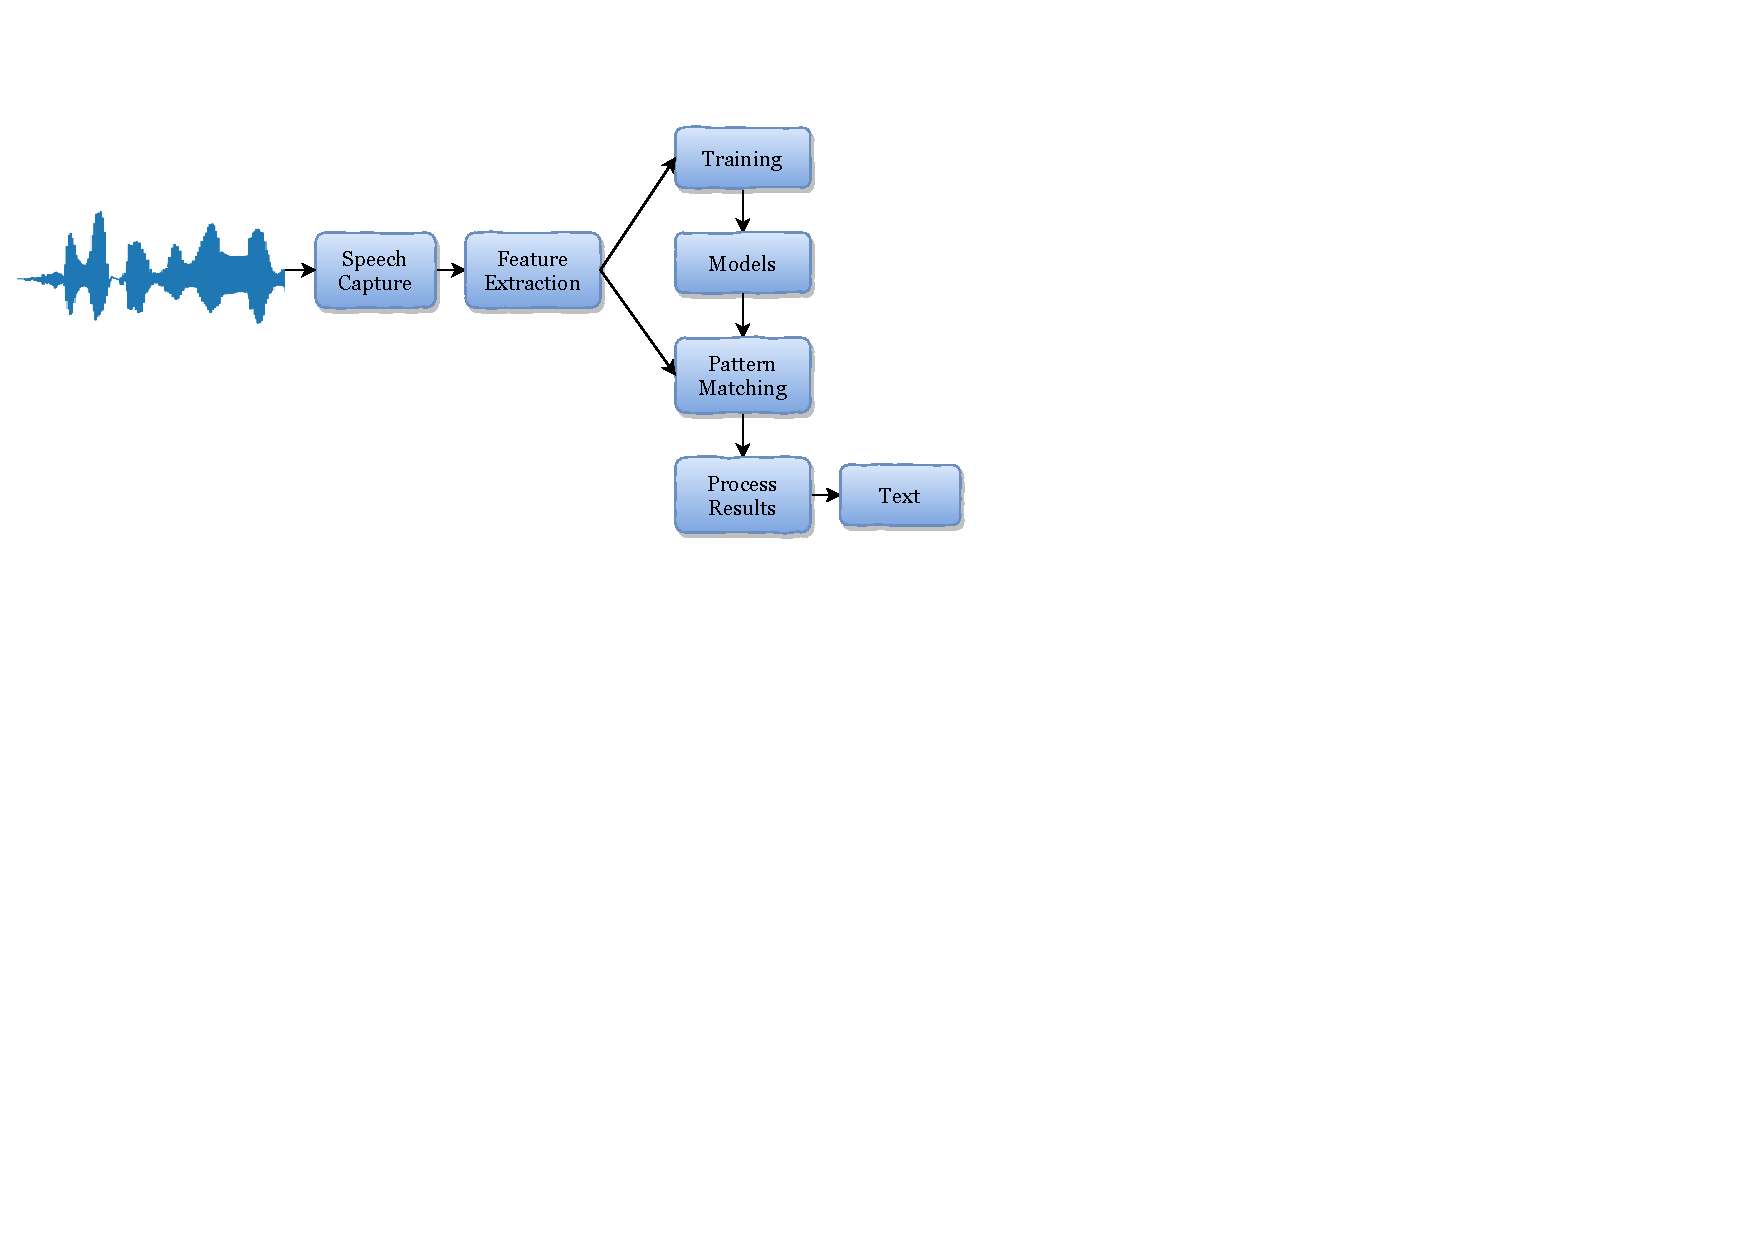
\includegraphics[scale=0.7]{Figures/speechProc}
\end{figure}
\end{frame}

\begin{frame}{Applications: Biometric Recognition}
\vspace{-6pt}
\begin{multicols}{2}
\begin{itemize}
\item Fingerprint
\item Eyes - Iris recognition
\item Face recognition, identification/verification
\item Speech recognition
\item Finger geometry recognition
\item Hand geometry recognition
\item Signature recognition
\item Eyes - Retina recognition
\item Fingerprint recognition
\item Typing recognition
\item Gait recognition
\item DNA identification
\end{itemize}
\end{multicols}
\begin{figure}
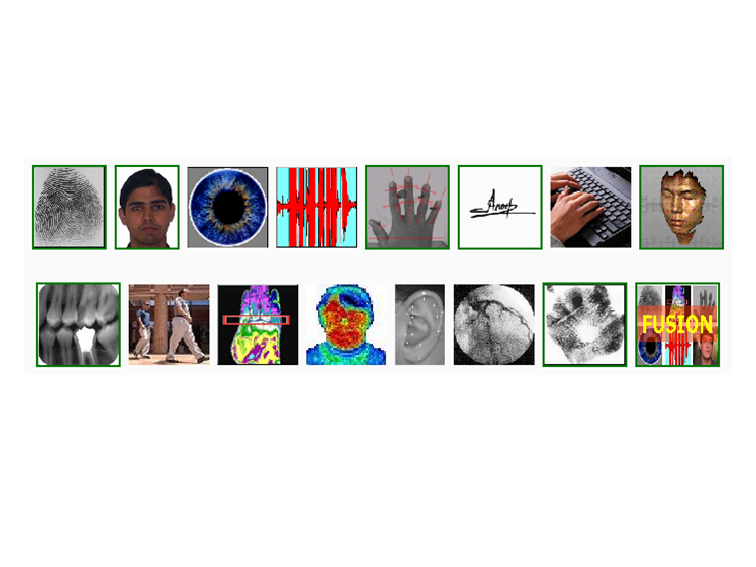
\includegraphics[scale=0.9]{BiometricRecognition}
\end{figure}
\end{frame}

\begin{frame}{Applications: Fingerprint Identification}
\begin{columns}
\begin{column}{6cm}
\begin{itemize}
\item No two people have the same fingerprints
\item Fingerprints can solve crimes.
\item Fingerprints are impressions created by ridges on the skin.
\item Ridges form before a baby is born and maintain their pattern thoughout life.
\item As we grow, the pattern gets larger, but does not changes.
\end{itemize}
\end{column}
\begin{column}{5cm}
\begin{figure}
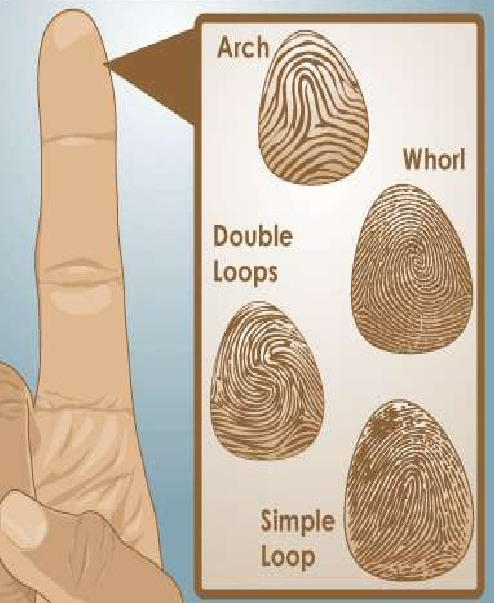
\includegraphics[scale=0.28]{Finger01.jpg}
\end{figure}
\end{column}
\end{columns}
\end{frame}

\begin{frame}{Applications: Fingerprint identification}
How Fingerprint scanners record identifies:
\vspace{1.8cm}
\begin{figure}
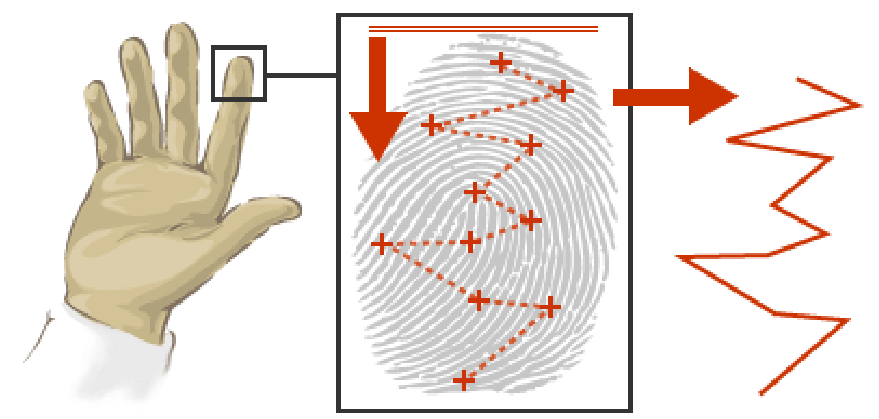
\includegraphics[scale=0.32]{Figures/Finger02.png}
\end{figure}
\begin{tikzpicture}[remember picture,overlay]
  \node [text width=3cm,minimum height=1cm,minimum width=2cm,execute at begin node=\setlength{\baselineskip}{10pt}] at (1.6,6.7) {{\small \textbf{1.} Inidividuals index finger is pressed onto scanner}};
   \node [text width=4cm,minimum height=1cm,minimum width=2cm,execute at begin node=\setlength{\baselineskip}{10pt}] at (5.5,6.7) {{\small \textbf{2.} Scanner reads unique pattern plotting specific distinctions (minutiae)}};
    \node [text width=4cm,minimum height=1cm,minimum width=2cm,execute at begin node=\setlength{\baselineskip}{10pt}] at (9.6,6.45) {{\small \textbf{3.} Points are linked forming a pattern recorded as an algorithm used for comparison}};
\end{tikzpicture}
\end{frame}

\begin{frame}{Applications: Face Recognition}
\begin{figure}
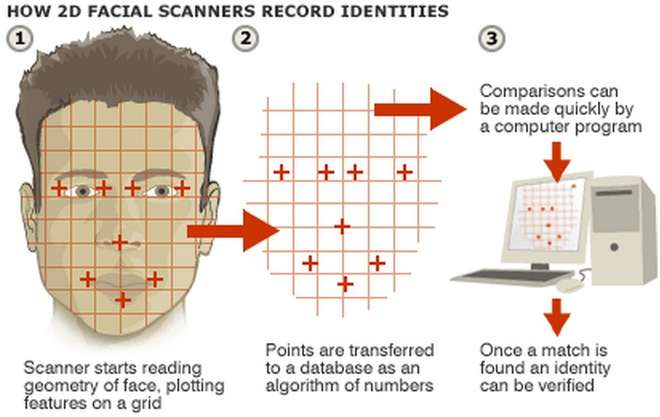
\includegraphics[scale=0.75]{FaceRecog.jpg}
\end{figure}
\end{frame}

\begin{frame}{Applications: Face Recognition}
\begin{figure}
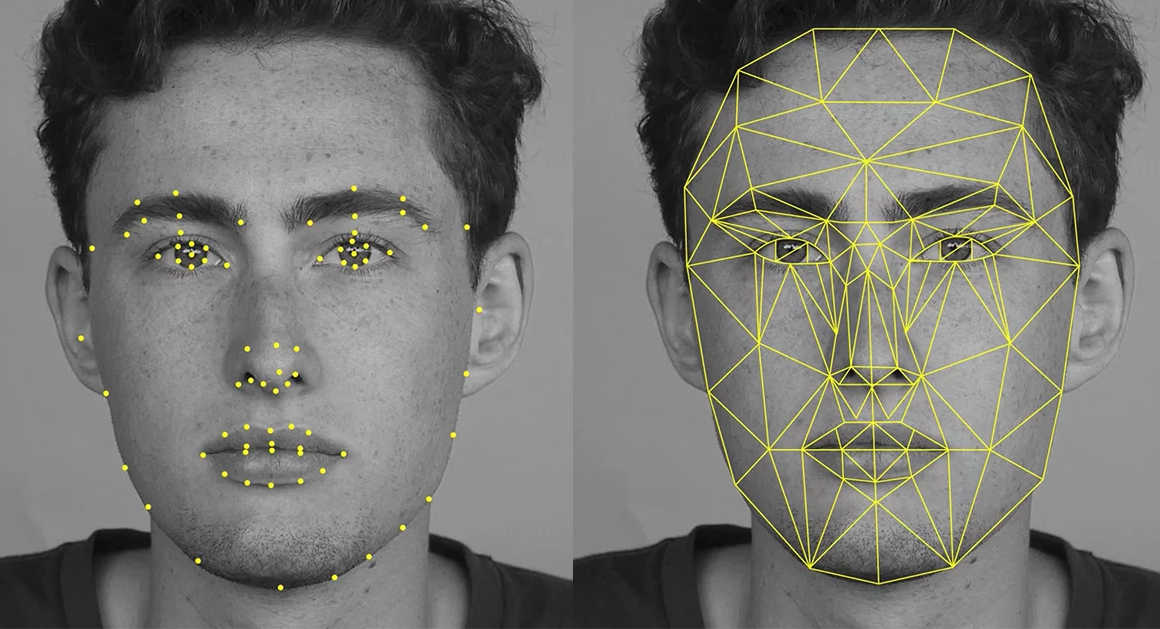
\includegraphics[scale=0.23]{FaceRecog01.png}
\end{figure}
\end{frame}

\begin{frame}{Applications: Optical Character Recognition (OCR)}
\begin{columns}
\begin{column}{5cm}
\begin{figure}
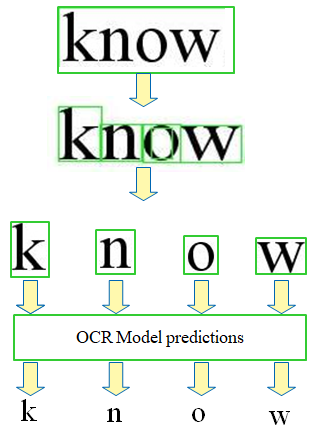
\includegraphics[height=6.3cm]{Figures/ocr.png}\\

\includegraphics[height=0.7cm]{Figures/ocr1.png}
\end{figure}
\end{column}
\begin{column}{6cm}
\begin{figure}
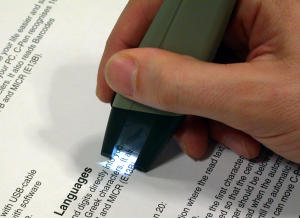
\includegraphics[height=1.5cm]{OCR02.jpg}
\end{figure}
\vspace{-0.5cm}
\begin{enumerate}
\item Differentiate word contours associated with Image.
\item Differentiate letter contours associated with word contours associated with word contour image.
\item Preprocess letter images according to trained OCR input
\item Consolidate predictions associated OCR model to text.
\end{enumerate}
\end{column}
\end{columns}
\end{frame}

\begin{frame}{Applications: DNA Identification}
\begin{figure}
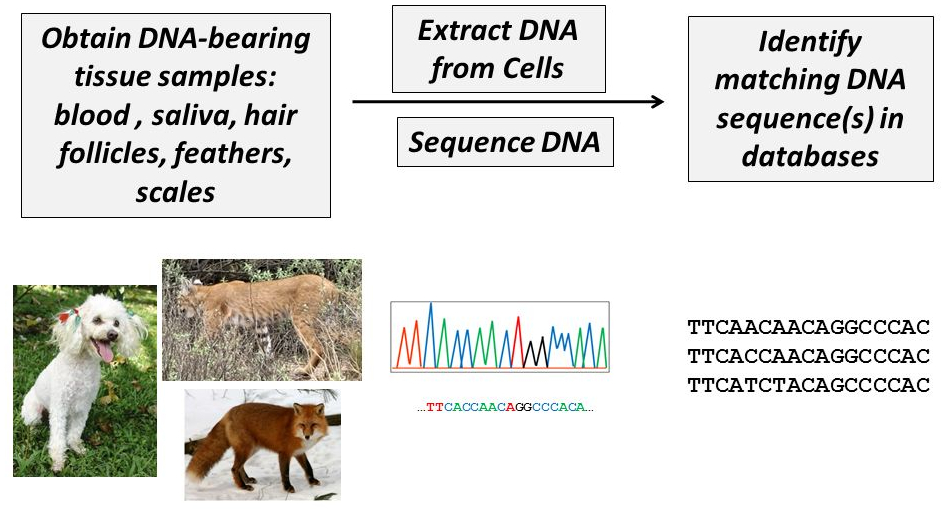
\includegraphics[scale=0.4]{DNA01.jpg}
\end{figure}
\end{frame}

\begin{frame}{Applications: Autonomous Navigation}
\begin{figure}
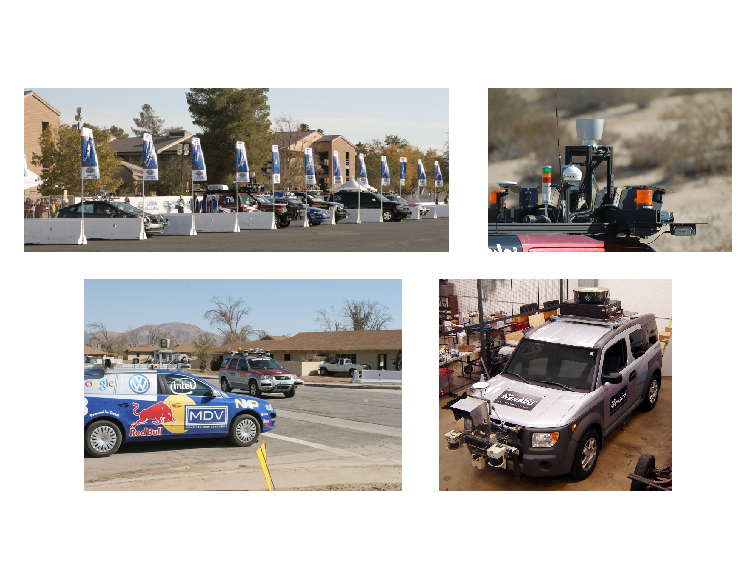
\includegraphics[scale=0.9]{AutoCar}
\end{figure}
\end{frame}

\begin{frame}{Applications: Cancer Detection}
\begin{figure}
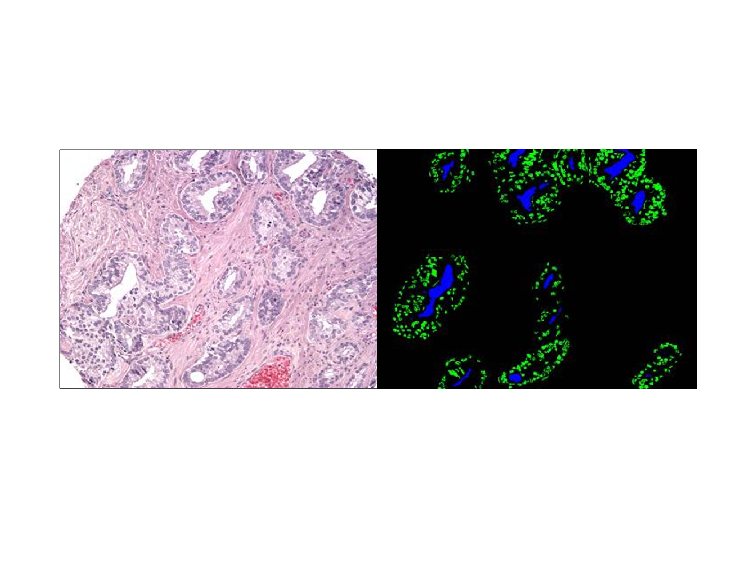
\includegraphics[scale=0.9]{CancerDetection}
\caption{Cancer detection and grading using microscopic tissue data}
\end{figure}
\end{frame}

\begin{frame}{Applications: Land Cover Detection}
\begin{figure}
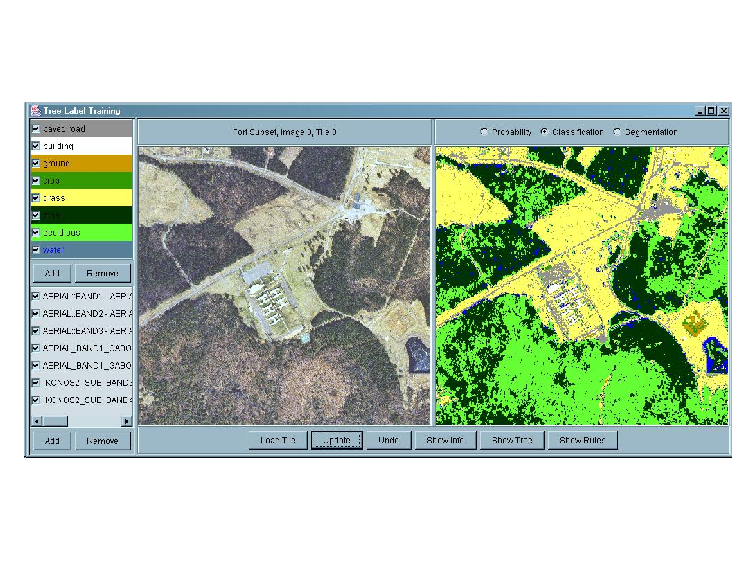
\includegraphics[scale=0.9]{LandCover}
\caption{Land cover classification using satellite image}
\end{figure}
\end{frame}

\begin{frame}{Applications: License Plate Recognition}
\begin{figure}
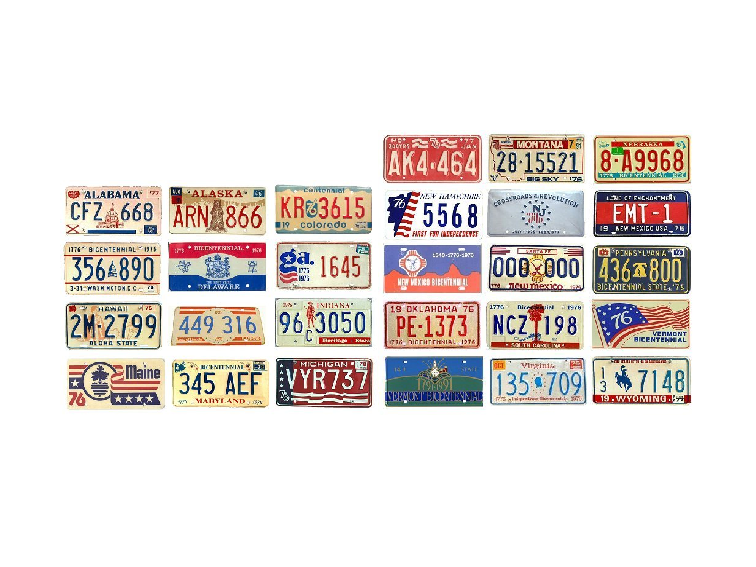
\includegraphics[scale=0.9]{LPlates}
\caption{License plate recognition: US license plates}
\end{figure}
\end{frame}

\section{An Example}
\subsection{}

\begin{frame}{}
\begin{variableblock}{\centering \Large \textbf{\vspace{4pt}\newline A classic example to understand Pattern Classification\vspace{4pt}}}{bg=slidecolor,fg=white}{bg=slidecolor,fg=white}
\end{variableblock}
\end{frame}

\begin{frame}{An Example}
\vspace{-4pt}
\begin{itemize}
\item ``Sorting incoming Fish on a conveyor according to species using optical sensing\nocite{duda2012pattern,Omer2018}"
\item Species
\begin{itemize}
\item Sea bass
\item Salmon
\end{itemize}
\begin{figure}
\centering
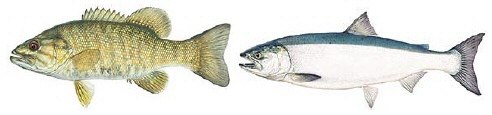
\includegraphics[scale=0.4]{FishImg.jpg}
\end{figure}
\item Set up a camera and take some sample image to extract features
\begin{itemize}
\item Length
\item Lightness
\item Width
\item Number and shape of fins
\item Position of the mouth, etc.
\end{itemize}
\item This is the set of all suggested features to explore for use in our classifier.
\end{itemize}
\end{frame}

\begin{frame}{An Example}
\begin{columns}
\begin{column}{6cm}
\begin{itemize}
\item What can cause problems during sensing?
\begin{itemize}
\item {\color{mycolor2}lighting conditions}, 
\item position of fish on the conveyor belt, 
\item camera noise, etc.
\end{itemize}
\item Use a segmentation operation to {\color{mycolor2}isolate fishes} from one another and from the {\color{mycolor2}background}.
\item Information from a single fish is sent to a {\color{mycolor1}feature extractor} whose purpose is to reduce the data by measuring certain features.
\item The features are passed to a classifier.
\end{itemize}
\end{column}
\begin{column}{5cm}
\begin{figure}
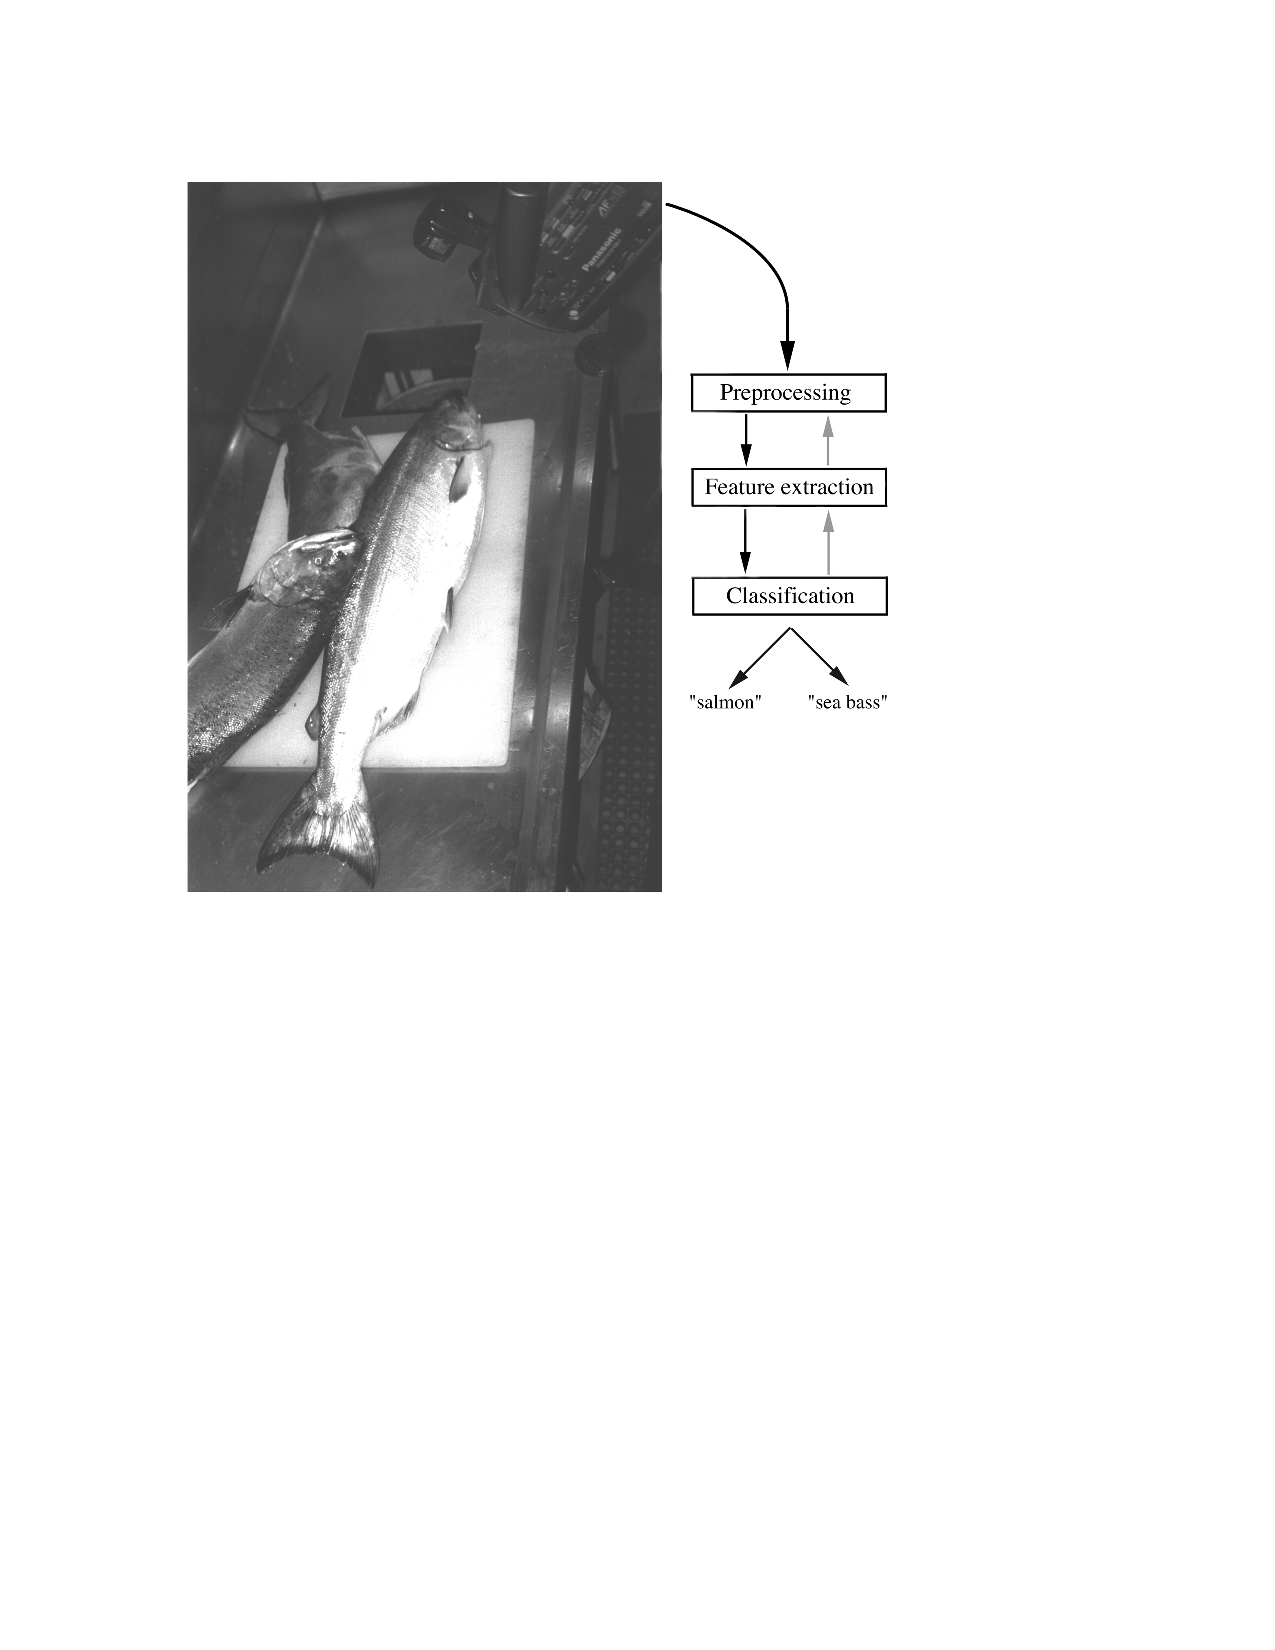
\includegraphics[scale=0.45]{Ch0214}
\end{figure}
\end{column}
\end{columns}
\end{frame}

%\begin{frame}{An Example}
%\begin{figure}
%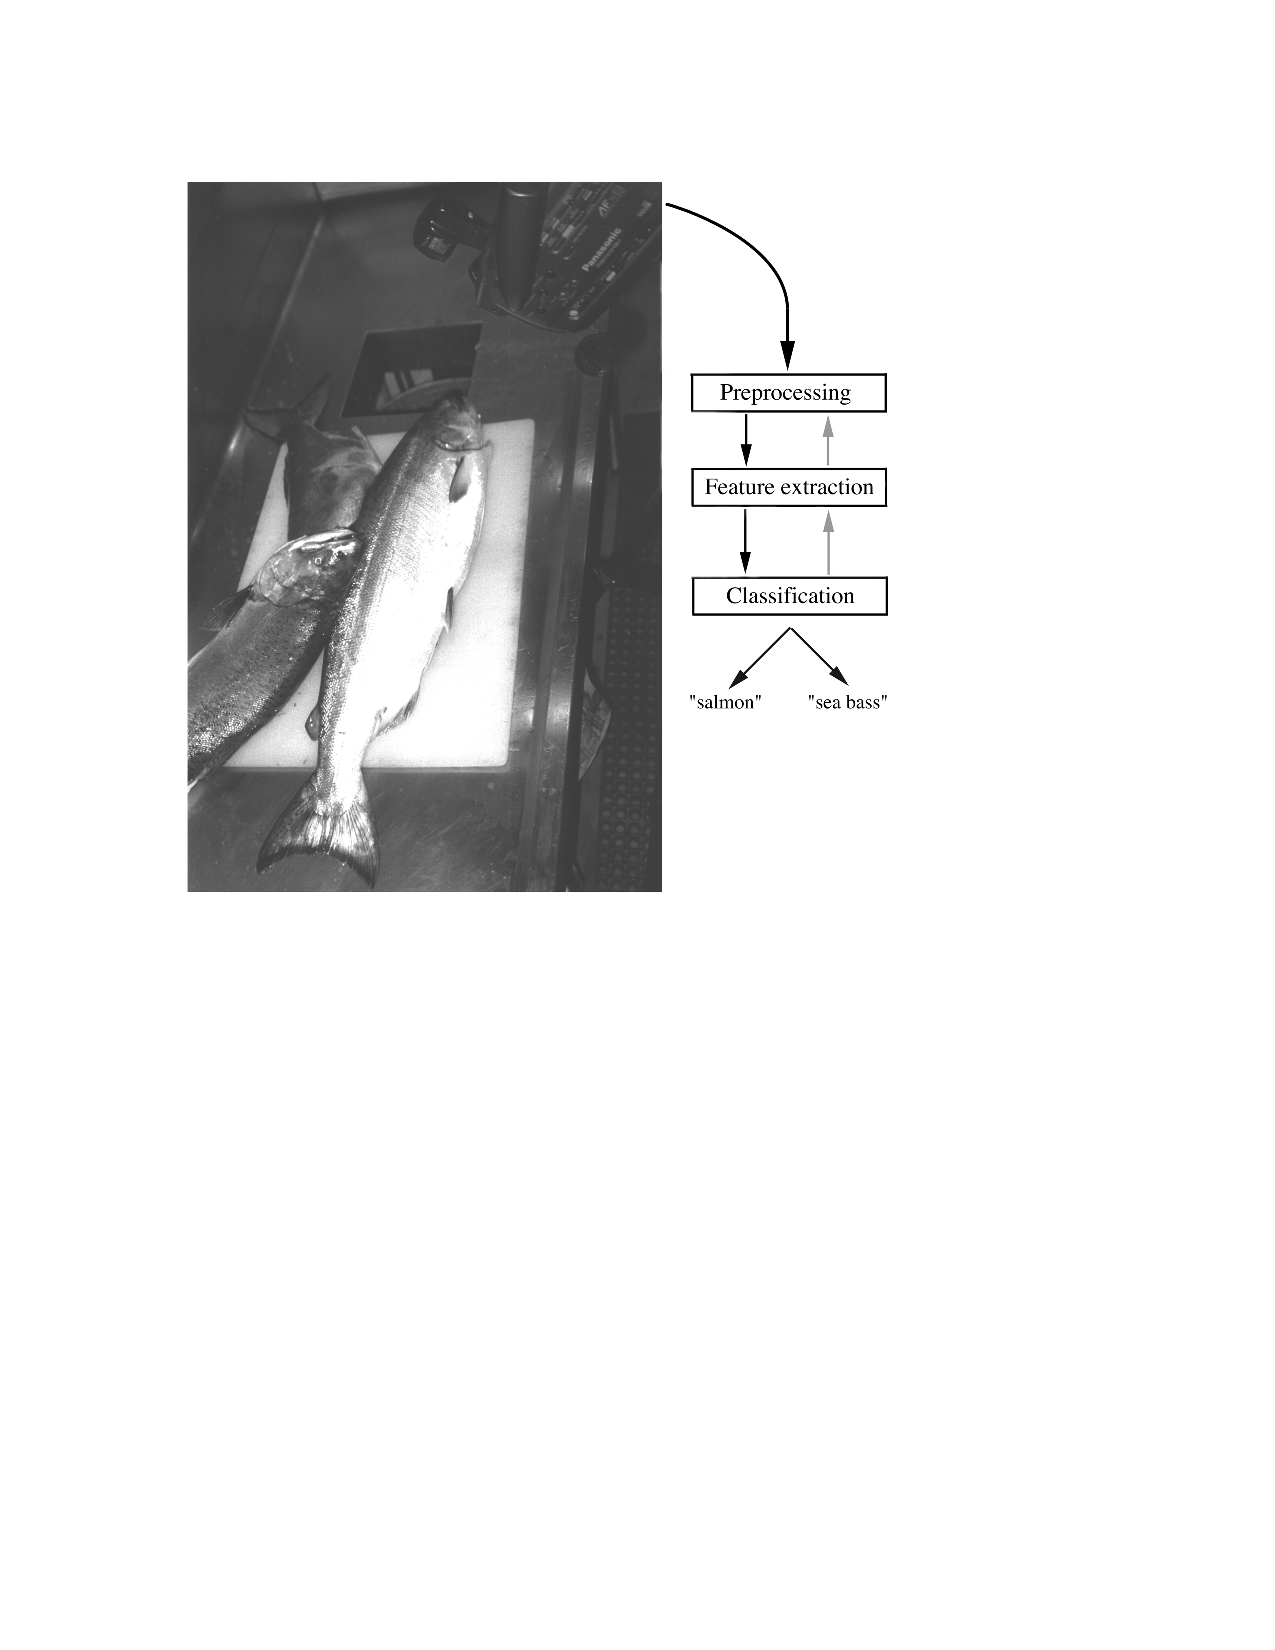
\includegraphics[scale=0.55]{Ch0214}
%\end{figure}
%\end{frame}

\begin{frame}{An Example: Classification}
\begin{itemize}
\item Select the length of the fish as a possible feature for discrimination
\end{itemize}
\begin{figure}
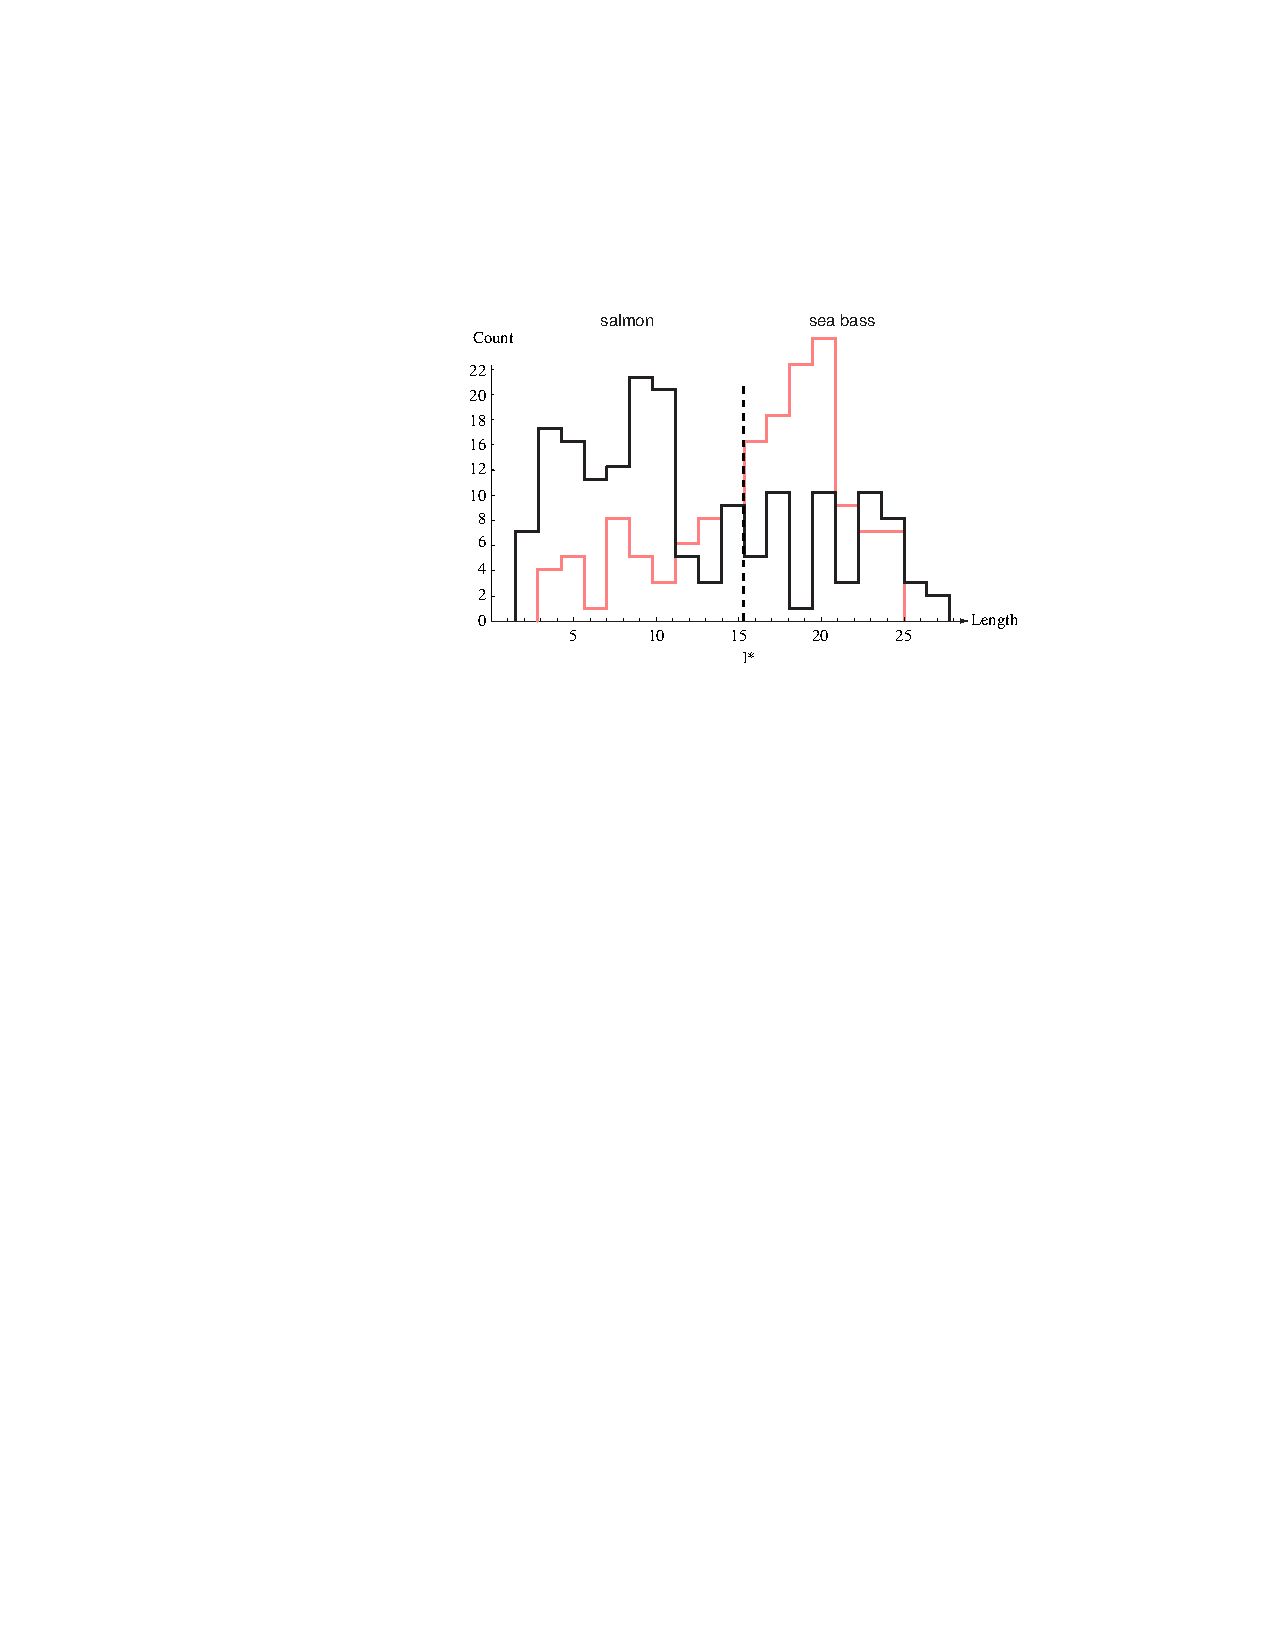
\includegraphics[scale=0.75]{Figures/Ch0101}
\caption{Histograms for the length feature for the two categories. No single threshold value $l^*$ (decision boundary) will serve to unambiguously discriminate between the two categories; using length alone, we will have some errors. The value $l*$ marked will lead to the smallest number of errors, on average.}
\end{figure}
\end{frame}

\begin{frame}{An Example: Classification}
\begin{itemize}
\item The length is a poor feature alone
\item Select the lightness as a possible feature
\end{itemize}
\begin{figure}
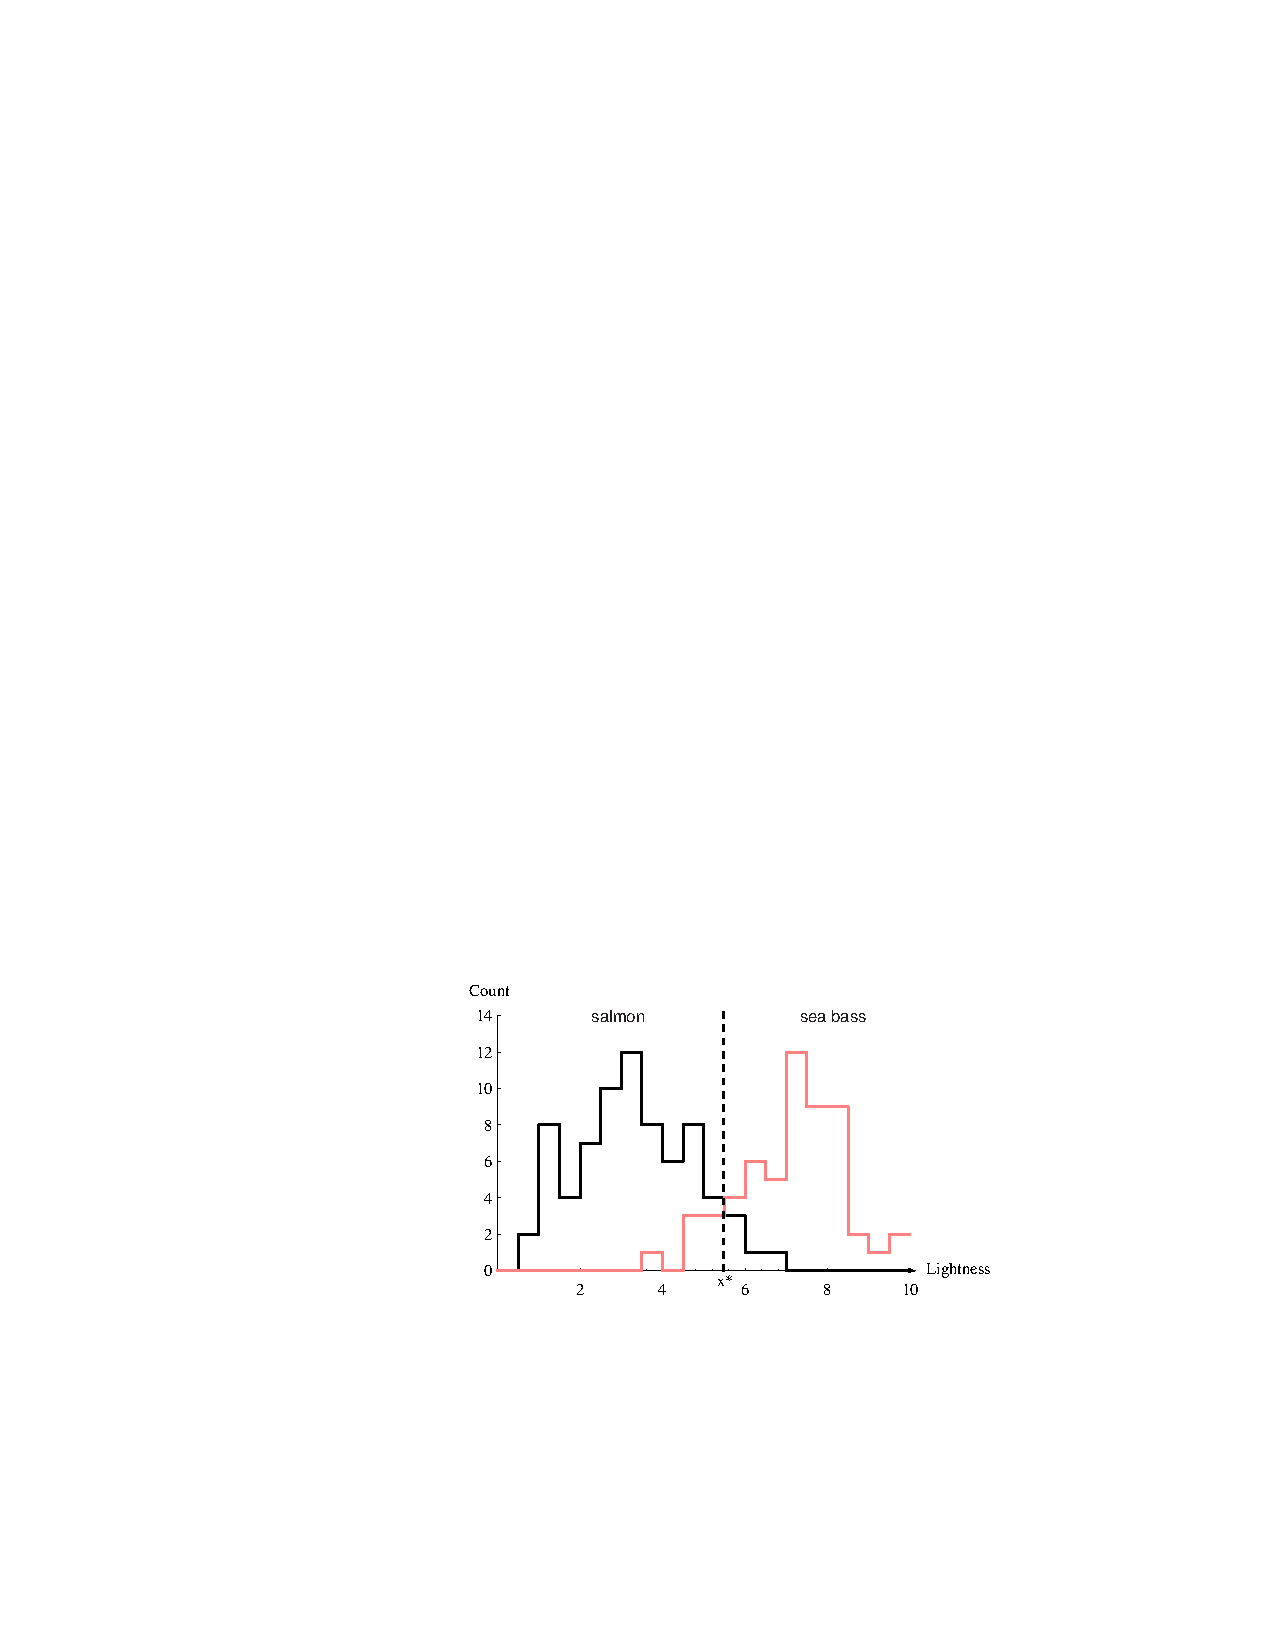
\includegraphics[scale=0.8]{Figures/Ch0102}
\caption{Histograms for the lightness feature for the two categories. No single threshold value $x^*$ (decision boundary) will serve to unambiguously discriminate between the two categories; using lightness alone, we will have some errors. The value $x^*$  marked will lead to the smallest number of errors, on average.}
\end{figure}
\end{frame}

\begin{frame}{Threshold decision boundary and cost relationship}
\begin{itemize}
\item Move our decision boundary toward smaller values of lightness in order to \textit{\color{mycolor2}minimize the cost} (reduce the number of sea bass that are classified salmon)\\
\vspace{14pt}
\begin{center}
{\Huge $\Downarrow$}\\
\vspace{14pt}
Task of decision theory
\end{center}
\end{itemize}
\end{frame}

\begin{frame}{An Example: Feature vector}
\begin{itemize}
\item Adopt the lightness and add the width of the fish
\item We can use two features in our decision:
\begin{itemize}
\item lightness: $x_1$
\item width: $x_2$
\end{itemize}
\item Each fish image is now represented as a point ({\color{mycolor2}feature vector}) ${\rm x}$ in two-dimensional  {\color{mycolor2}feature space}.
\end{itemize}
\vspace{-0.5cm}
\begin{columns}
\begin{column}{6cm}
\begin{figure}
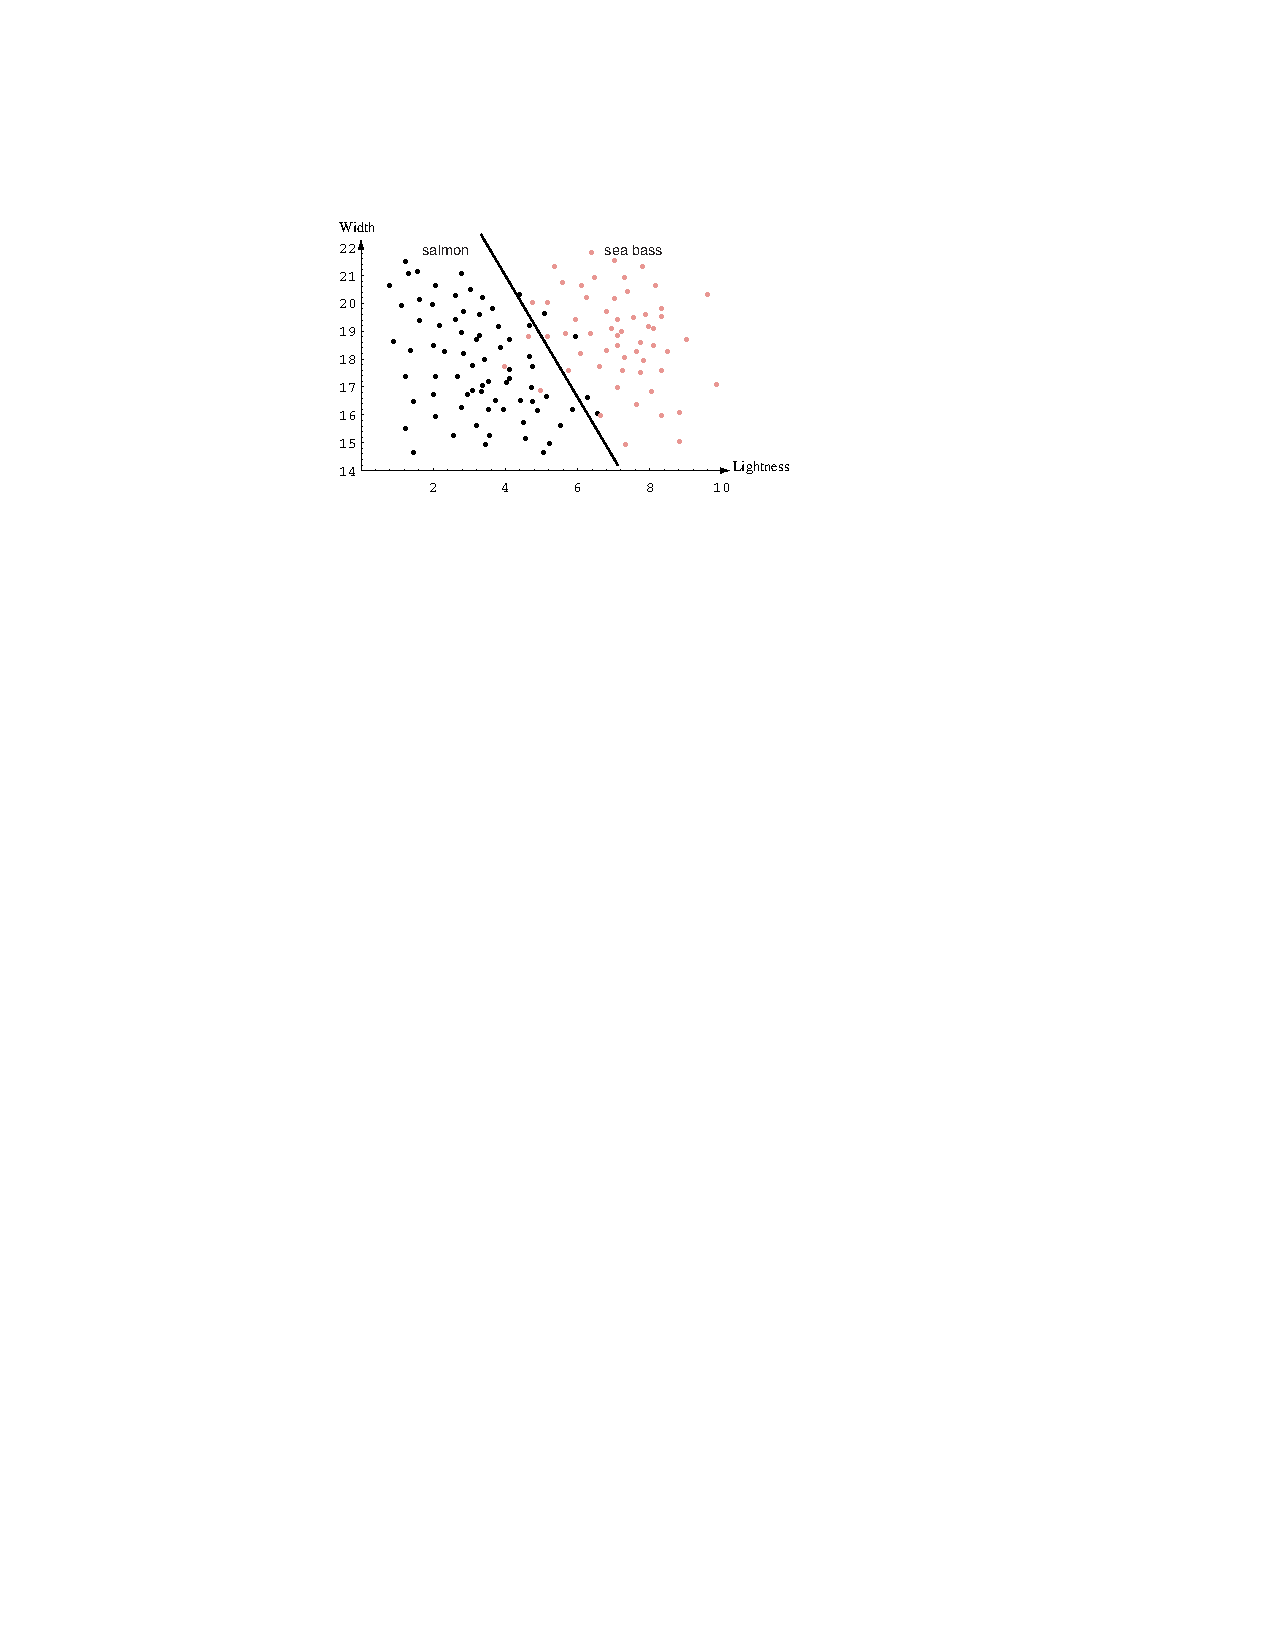
\includegraphics[scale=0.8]{Ch0103}
\end{figure}
\end{column}
\begin{column}{4cm}
$~~~{\rm x}=[x_1~~~~x_2]^T$\\
~~~~~~~~~$\downarrow$~~~~~$\downarrow$\\
Lightness~~ Width
\end{column}
\end{columns}
\end{frame}

\begin{frame}{An Example: Feature vector}
\begin{itemize}
\setlength{\itemsep}{12pt}
\item We might add other features that are not correlated with the ones we already have. A precaution should be taken not to reduce the performance by adding such ``noisy features''.
\item Does adding more features always improve the results?
\begin{itemize}
\item unreliable features.
\item Be careful about correlations with existing features.
\item Be careful about measurement costs.
\item Be careful about noise in the measurements.
\end{itemize} 
\item Is there some \textit{\color{mycolor2}curse} for working in very high dimensions?
\end{itemize}
\end{frame}

\begin{frame}{An Example: Feature vector}
\begin{itemize}
\item Ideally, the best decision boundary should be the one which provides an optimal performance.
\begin{figure}
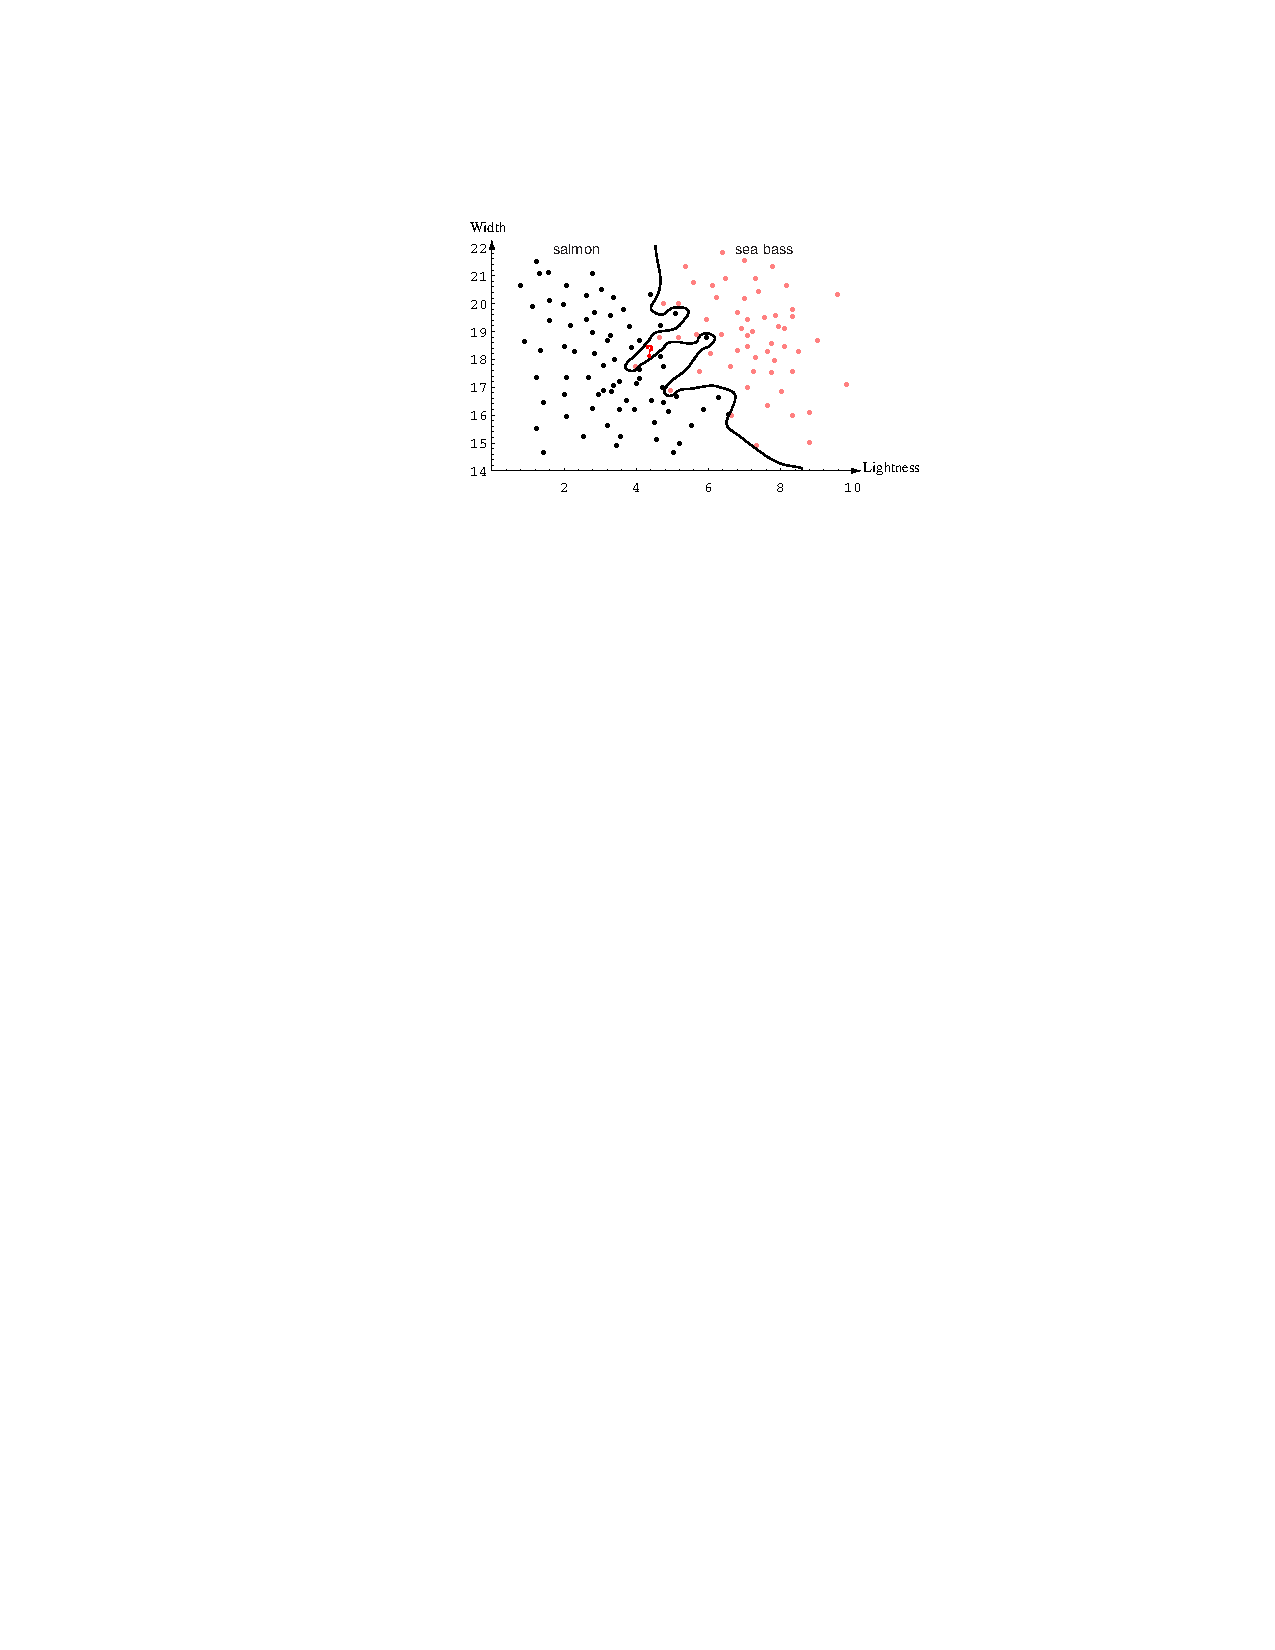
\includegraphics[scale=1.1]{Ch0104}
\end{figure}
\end{itemize}
\end{frame}

\begin{frame}{An Example: Issue of generalization}
\begin{itemize}
\item How can we mange the \textit{\color{mycolor2}tradeoff} between complexity of decision rules and their performance to unknown samples?
\item Our satisfaction is premature because the central aim of designing a classifier is to correctly classify novel input\\
\vspace{14pt}
\begin{center}
{\Huge $\Downarrow$}\\
\vspace{14pt}
Issue of generalization
\end{center}
\end{itemize}
\end{frame}

\begin{frame}{An Example: Decision Boundary}
\begin{figure}
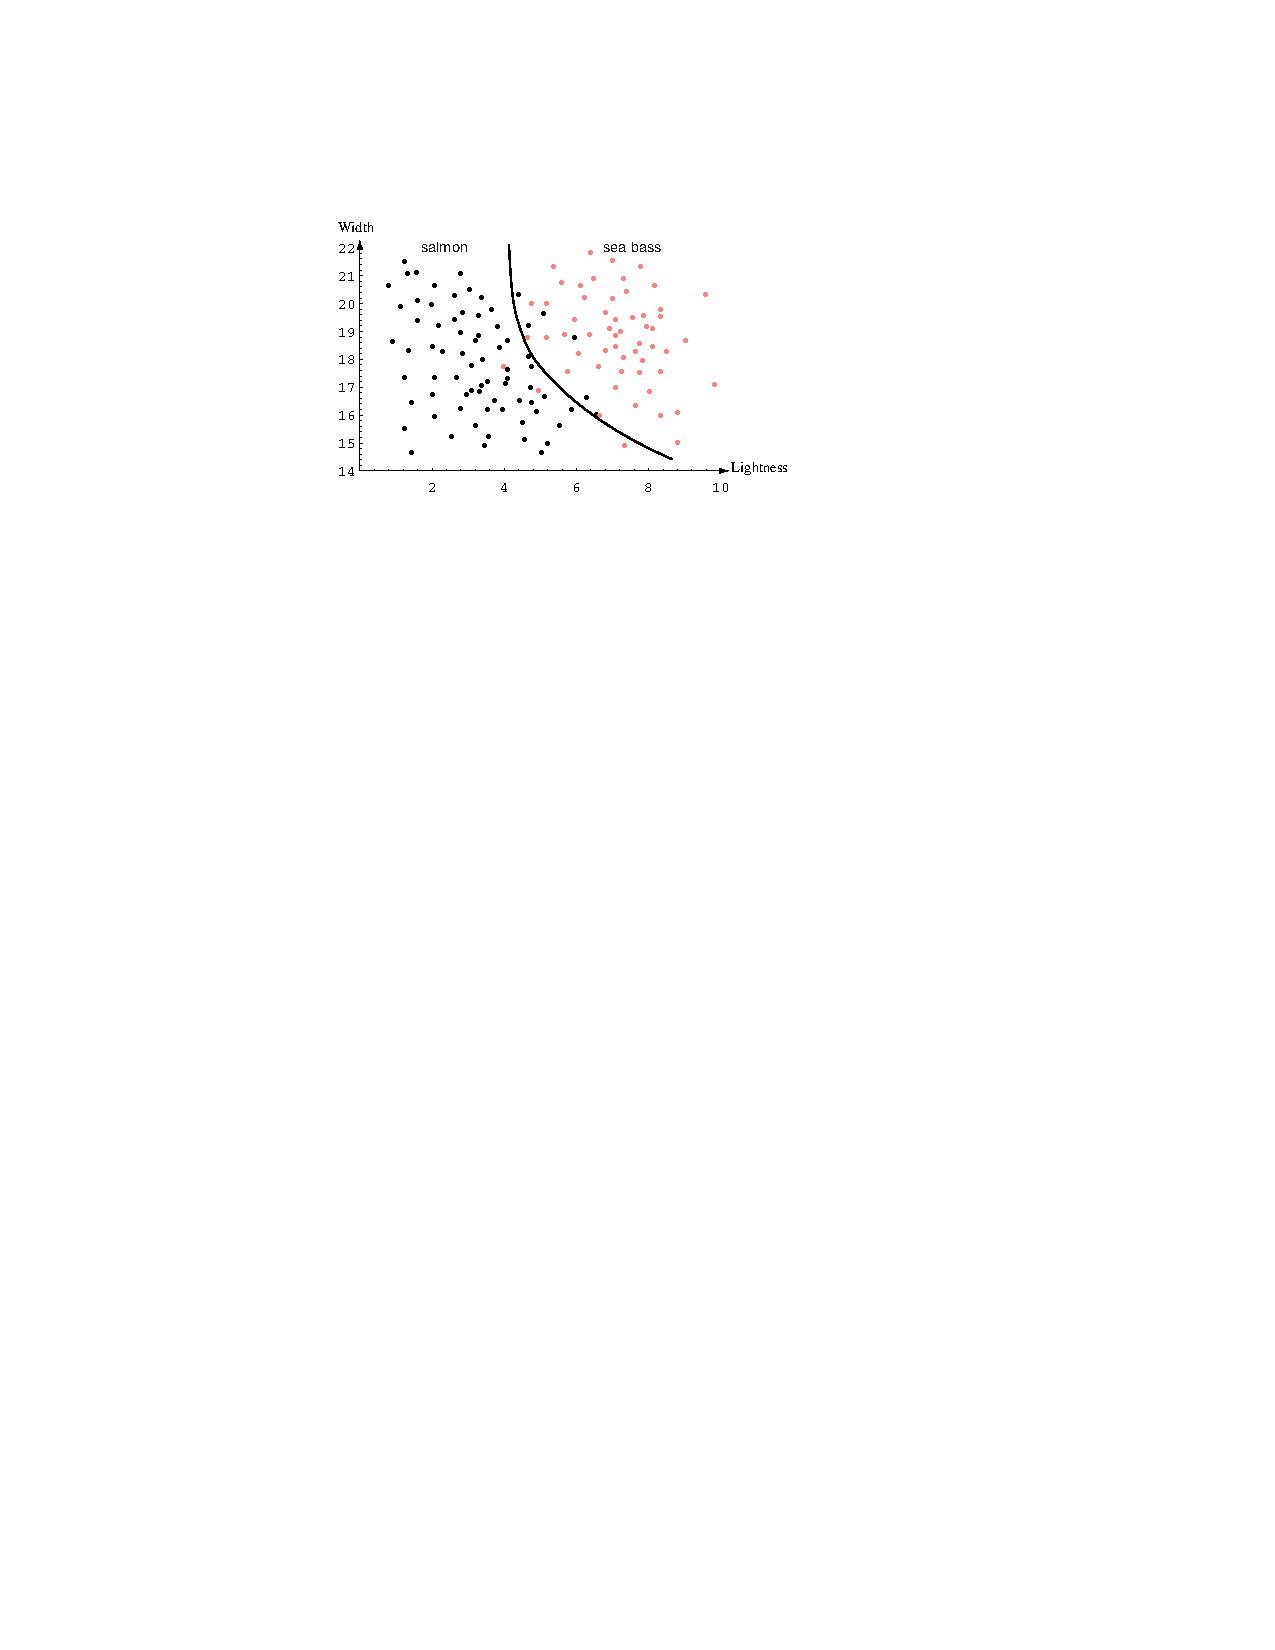
\includegraphics[scale=1.1]{Figures/Ch0105}
\caption{The decision boundary shown might represent the optimal trade of between performance on the training set and simplicity of classifier.}
\end{figure}
\end{frame}

\begin{frame}{More on Complexity}
\begin{figure}
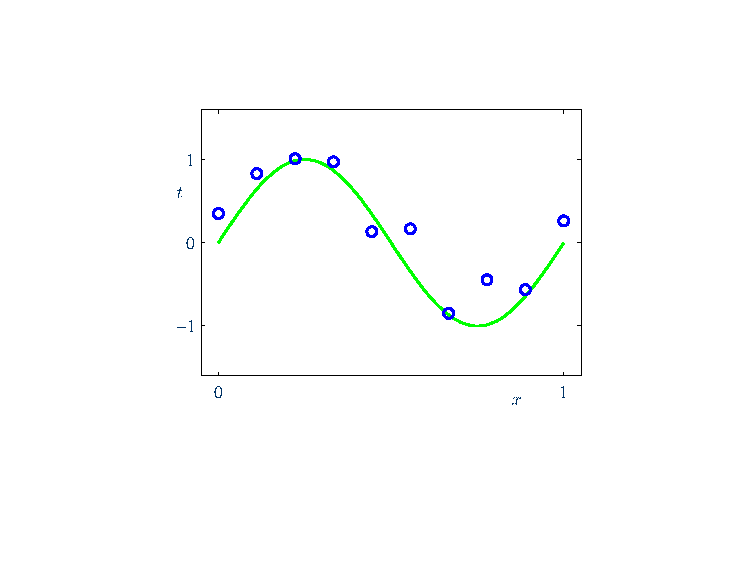
\includegraphics[scale=1]{Reg01}
\caption{Regression example: plot of 10 sample points for the input variable $x$ along with the corresponding target variable $t$. Green curve is the true function that generated the data.}
\end{figure}
\end{frame}

\begin{frame}{More on Complexity}
\begin{figure}
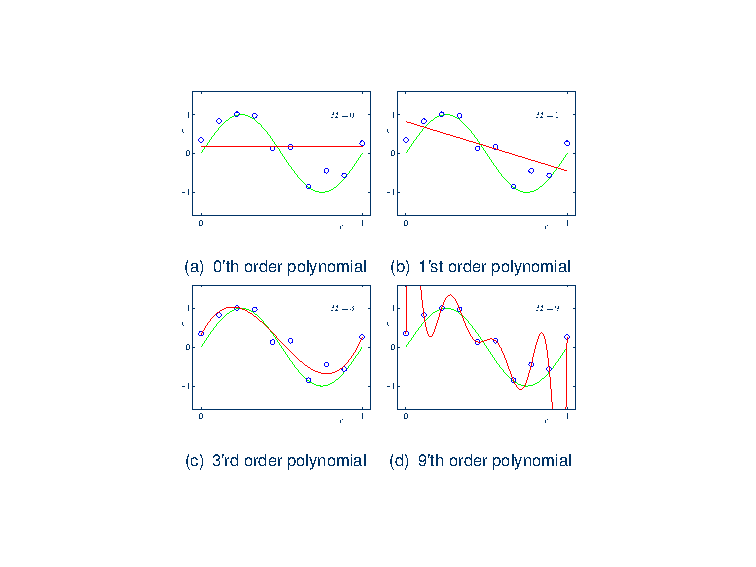
\includegraphics[scale=0.9]{Reg02}
\caption{Polynomial curve fitting: plots of polynomials having various orders, shown as red curves, fitted to the set of 10 sample points}
\end{figure}
\end{frame}

\begin{frame}{More on Complexity}
\begin{figure}
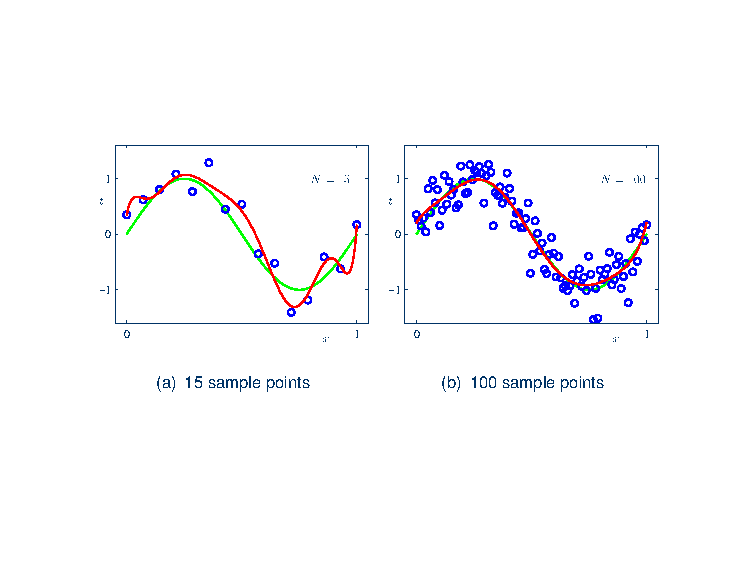
\includegraphics[scale=1]{Reg03}
\caption{Polynomial curve fitting: plots of 9'th order polynomials fitted to 15 and 100 sample points.}
\end{figure}
\end{frame}

\section[PR Systems]{Pattern Recognition System}
\subsection{}

\begin{frame}{}
\begin{variableblock}{\centering \Large \textbf{\vspace{4pt}\newline Pattern recognition system and design cycle\vspace{4pt}}}{bg=slidecolor,fg=white}{bg=slidecolor,fg=white}
\end{variableblock}
\end{frame}


\begin{frame}{Pattern Recognition Models}
There are three main models of pattern recognition:
\setlength{\itemsep}{12pt}
\begin{itemize}
\item {\color{mycolor1}Statistical:} 
\begin{itemize}
\item to identify where specific piece belongs (for example, whether it is a cake or not).
\item use of statistics to learn from examples.
\end{itemize}


\item {\color{mycolor1}Syntactic/Structural:} 
\begin{itemize}
\item to define a more complex relationship between elements taking into account more complex interrelationships between attributes.
\item Looks at clear structure in the patterns.
\item An example of this would be diagnosis of the heart with ECG measurements.
\end{itemize}
\item {\color{mycolor1}Template Matching:}
\begin{itemize}
\item To match the object's features with the predefined template and identify the object by proxy. 
\item One of the uses of such model is plagiarism checking.
\end{itemize} 
\end{itemize}
\end{frame}

\begin{frame}{Pattern Recognition Systems}
\begin{figure}
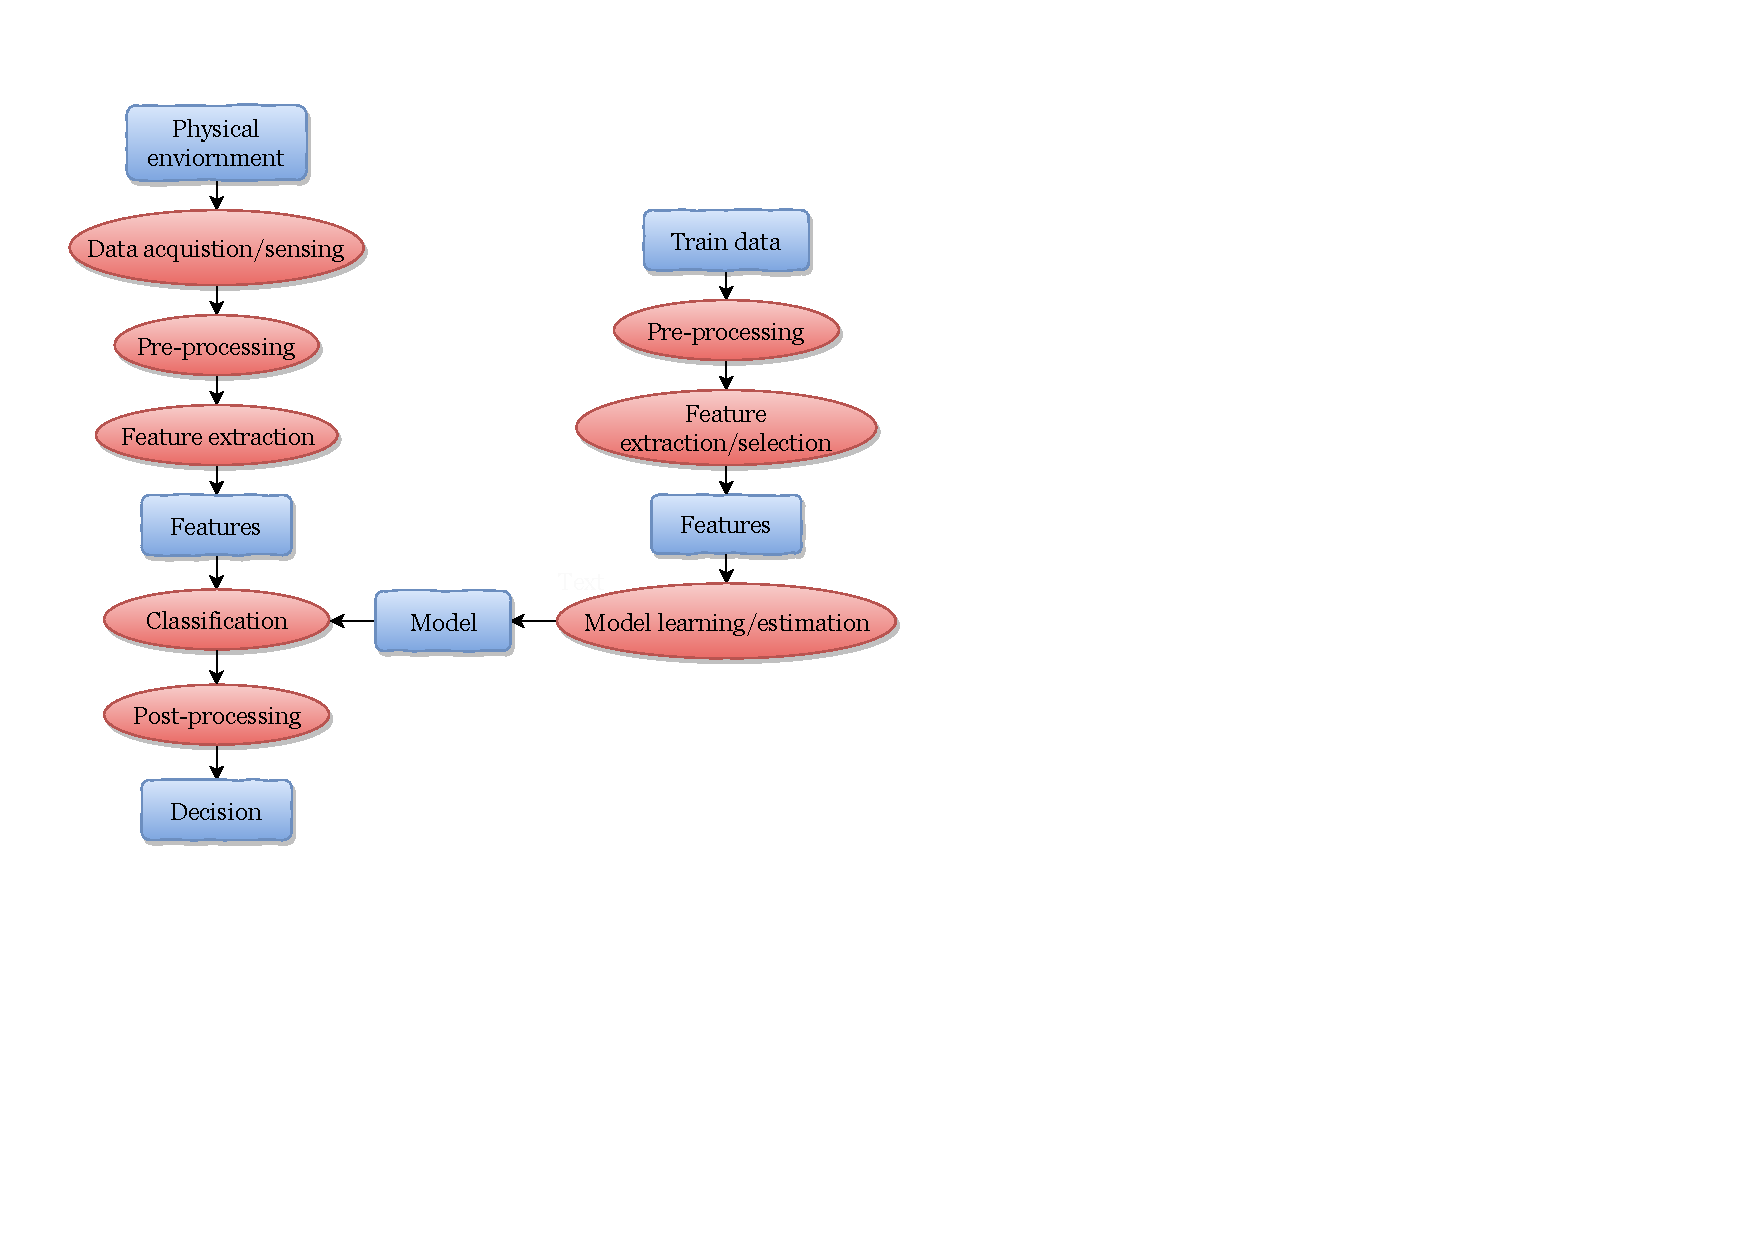
\includegraphics[width=7cm]{Figures/PRsystem2}
\caption{Object/Process diagram of a pattern recognition system}
\end{figure}
\end{frame}

\begin{frame}{Pattern Recognition Systems}
\begin{itemize}
\setlength{\itemsep}{6pt}
\item {\color{mycolor2}Data acquisition and sensing:}
\begin{itemize}
\item Use of transducer (camera or microphone)
\item Measurements of physical variables.
\item Important issues: bandwidth, resolution, sensitivity,
distortion, SNR, latency, etc.
\end{itemize}
\item {\color{mycolor2}Pre-processing:}
\begin{itemize}
\item  Removal of noise in data.
\item Isolation of patterns of interest from the background.
\item Segmentation and grouping
\end{itemize}
\item {\color{mycolor2}Feature extraction:}
\begin{itemize}
\item Finding a new representation in terms of features.
\item Features should be well separated and should not overlap (Discriminative features )
\item Invariant features with respect to translation, rotation and scale.
\item Depends on the characteristics of the problem domain. Simple to extract, invariant to irrelevant transformation insensitive to noise.
\end{itemize} 
\end{itemize}
\end{frame}

\begin{frame}{Pattern Recognition Systems}
\begin{itemize}
\setlength{\itemsep}{6pt}
\item {\color{mycolor2} Model learning and estimation:}
\begin{itemize}
\item Learning a mapping between features and pattern groups and categories.
\item Unsatisfied with the performance of classifier and want to jump to another class of model
\end{itemize}
\item {\color{mycolor2}Classification:}
\begin{itemize}
\item  Using features and learned models to assign a pattern to a category.
\end{itemize}
\item {\color{mycolor2}Post-processing:}
\begin{itemize}
\item Evaluation of confidence in decisions.
\item Exploitation of context to improve performance.
\item Combination of experts.
\end{itemize} 
\end{itemize}
\end{frame}

\section{Design Cycle}
\subsection{}

\begin{frame}{The Design Cycle}
\begin{figure}
\includegraphics[width=\textwidth]{Figures/DesignCycle}
\caption{Design cycle}
\end{figure}
\begin{itemize}
\item {\color{mycolor2}Data Collection}
\begin{itemize}
\item Collecting training and testing data.
\item How do we know when we have collected an adequately large and representative set of examples for training and testing the system?
\end{itemize}
\end{itemize}
\vspace{2cm}
\end{frame}

\begin{frame}{The Design Cycle}
\begin{figure}
\includegraphics[width=\textwidth]{Figures/DesignCycle}
\caption{Design cycle}
\end{figure}
\vspace{-20pt}
\begin{itemize}
\setlength{\itemsep}{12pt}
\item {\color{mycolor2}Feature Selection}
\begin{itemize}
\setlength{\itemsep}{3pt}
\item Domain dependence and prior information.
\item Computational cost and feasibility.
\item Discriminative features.
\begin{itemize}
\item Similar values for similar patterns.
\item Different values for different patterns.
\end{itemize}
\item Invariant features with respect to translation, rotation and
scale.
\item Robust features with respect to occlusion, distortion,
deformation, and variations in environment.
\end{itemize}
\end{itemize}
\end{frame}

\begin{frame}{The Design Cycle}
\begin{figure}
\includegraphics[width=\textwidth]{Figures/DesignCycle}
\caption{Design cycle}
\end{figure}
\vspace{-20pt}
\begin{itemize}
\item {\color{mycolor2}Model selection}
\begin{itemize}
\setlength{\itemsep}{3pt}
\item Domain dependence and prior information.
\item Definition of design criteria.
\item Parametric vs. non-parametric models.
\item Handling of missing features.
\item Computational complexity.
\item Types of models: templates, decision-theoretic or statistical, syntactic or structural, neural, and hybrid.
\item How can we know how close we are to the true model
underlying the patterns?
\end{itemize}
\end{itemize}
\end{frame}

\begin{frame}{The Design Cycle}
\begin{figure}
\includegraphics[width=\textwidth]{Figures/DesignCycle}
\caption{Design cycle}
\end{figure}
\begin{itemize}
\item {\color{mycolor2}Training}
\begin{itemize}
\setlength{\itemsep}{3pt}
\item How can we learn the rule from data?
\item Supervised learning: a teacher provides a category label or
cost for each pattern in the training set.
\item Unsupervised learning: the system forms clusters or natural groupings of the input patterns.
\item Reinforcement learning: no desired category is given but the teacher provides feedback to the system such as the
decision is right or wrong.
\end{itemize}
\end{itemize}
\end{frame}

\begin{frame}{The Design Cycle}
\begin{figure}
\includegraphics[width=\textwidth]{Figures/DesignCycle}
\caption{Design cycle}
\end{figure}
\vspace{-12pt}
\begin{itemize}
\setlength{\itemsep}{12pt}
\item {\color{mycolor2}Evaluation}
\begin{itemize}
\setlength{\itemsep}{2pt}
\item How can we estimate the performance with training
samples?
\item How can we predict the performance with future data?
\item Problems of overfitting and generalization.
\end{itemize}
\item {\color{mycolor2}Computational Complexity}
\begin{itemize}
\setlength{\itemsep}{2pt}
\item What is the trade-off between computational ease and performance?
\item How an algorithm scales as a function of the number of features, patterns or categories?
\end{itemize}
\end{itemize}
\end{frame}

\begin{frame}{Different Learning Approaches}
\begin{itemize}
\setlength{\itemsep}{8pt}
\item {\color{mycolor2}Supervised learning/Classification}
\begin{itemize}
\item A teacher provides a category label or cost for each pattern in the training set
\end{itemize}
\item {\color{mycolor2}Unsupervised learning/Clustering}
\begin{itemize}
\item The system forms clusters or "natural groupings" of the input pattern (no explicit teacher)
\end{itemize}
\item {\color{mycolor2}Semi-supervised learning}
\begin{itemize}
\item Semi-supervised learning is the problem of learning from examples for which you have labels for only a (small) subset.
\end{itemize}
\item {\color{mycolor2}Reinforcement learning}
\begin{itemize}
\item Learning with critic, no desired category is known; instead, the only teaching feedback is that the tentative category is right or wrong. It utilizes reward function to learn. Ex: Autonomous driving
\end{itemize}
\end{itemize}
\end{frame}

\section{References}
\subsection{}
\begin{frame}[allowframebreaks]{References}
\linespread{1}
\footnotesize
\printbibliography[heading=none]
\end{frame}
{
\setbeamertemplate{logo}{}
\makeatletter
\setbeamertemplate{footline}{
        \leavevmode%
  
  % First line.
  \hbox{%
  \begin{beamercolorbox}[wd=.2\paperwidth,ht=\beamer@decolines@lineup,dp=0pt]{}%
  \end{beamercolorbox}%
  \begin{beamercolorbox}[wd=.8\paperwidth,ht=\beamer@decolines@lineup,dp=0pt]{lineup}%
  \end{beamercolorbox}%
  } %
  % Second line.
  \hbox{%
  \begin{beamercolorbox}[wd=\paperwidth,ht=\beamer@decolines@linemid,dp=0pt]{linemid}%
  \end{beamercolorbox}%
  } %
  % Third line.
  \hbox{%
  \begin{beamercolorbox}[wd=.1\paperwidth,ht=\beamer@decolines@linebottom,dp=0pt]{}%
  \end{beamercolorbox}%
  \begin{beamercolorbox}[wd=.9\paperwidth,ht=\beamer@decolines@linebottom,dp=0pt]{linebottom}%
  \end{beamercolorbox}%
  }%
        }
\makeatother

\begin{frame}
\centering
\includegraphics[width=0.4\paperwidth]{queries.jpg}\\
\includegraphics[width=0.5\paperwidth]{thank_you.png}
\end{frame}
}

